\documentclass[pt12]{beamer}
%\documentclass[pt12,externalviewer]{beamer}

\usepackage{amssymb}
%\usepackage{rotating}
%\usepackage{amsmath}
\usepackage{tikz}
%\usepackage{beamergraphics}
\usepackage[english]{babel}
\usepackage[latin1]{inputenc}
\usepackage[T1]{fontenc}
\usepackage{cleveref}

%\usepackage[absolute,overlay]{textpos}
%\usepackage{pdfcolparallel}

%\usepackage{tcolorbox}
%\tcbuselibrary{fitting}

\usepackage{lipsum}

%\usepackage{subfig}
\usepackage{caption}
\usepackage{subcaption}

\usefonttheme{professionalfonts}
\usepackage{stmaryrd}

\definecolor{BBB}{rgb}{0.2,0.2,0.7} % UBC Blue (primary)
\definecolor{SSCgreen}{HTML}{a2da7b} % green as in the SSC logo (primary)
\definecolor{SSCdarkgreen}{HTML}{437024}
\definecolor{SSCred}{HTML}{d5685d}   % red   as in the SSC logo (primary)
\definecolor{SSCdarkred}{HTML}{bf2413}


\mode<presentation>
{
%  \usetheme{Warsaw} 
  \usetheme{Madrid}
%  \usetheme{Montpellier}
%  \usetheme{Marburg} 
  \usecolortheme[named=BBB]{structure}
  \setbeamercolor{alerted text}{fg=SSCdarkred}
  \setbeamercovered{transparent}
  \setbeamertemplate{section in toc}[ball unnumbered]
}

%\setbeamertemplate{footline}{\hfill\insertframenumber/\inserttotalframenumber} 

\expandafter\def\expandafter\insertshorttitle\expandafter{%
  \insertshorttitle\hfill%
  \insertframenumber\,/\,\inserttotalframenumber}

\newcommand{\backupbegin}{
   \newcounter{framenumberappendix}
   \setcounter{framenumberappendix}{\value{framenumber}}
}
\newcommand{\backupend}{
   \addtocounter{framenumberappendix}{-\value{framenumber}}
   \addtocounter{framenumber}{\value{framenumberappendix}} 
}

\newcommand{\refer}[1]{%
   \begin{flushright}
      {\alert{\tiny #1}}
   \end{flushright}}
  
\newcommand{\lrefer}[1]{%
   \begin{flushleft}
      {\alert{\tiny #1}}
   \end{flushleft}}
  
\newcommand{\param}[1]{%
   \begin{flushright}
      {\small #1}
   \end{flushright}
   \vspace{-1.5\baselineskip}
}

\newcommand{\sech}{\mathop{\rm sech}\nolimits}
\newcommand{\sgn}{\mathop{\rm sgn}\nolimits}
\newcommand{\etal}{{\em et al.}}


\newtheorem{observation}{Observation}
\newtheorem{proposition}{Proposition}
\newtheorem{cor}{Corollary}

\newcommand{\prob}[0]{P}

\newcommand{\lop}[0]{\mathcal{L}}
\newcommand{\lopd}[0]{\mathcal{L}_\Delta}
\newcommand{\lopdt}[0]{\mathcal{L}_{\Delta}}
\newcommand{\usol}[0]{\underline{\uvec{u}}_\Delta}
\newcommand{\usoldt}[0]{\underline{\uvec{u}}_\Delta}

\newcommand{\uex}[0]{\underline{\uvec{u}}^{ex}}
\newcommand{\up}[0]{\underline{\uvec{u}}^{(p)}}

\newcommand{\usoldto}[0]{\tilde{\underline{\uvec{u}}}_\Delta}

\newcommand{\uapp}[0]{\uvec{u}_h}
\newcommand{\wapp}[0]{w_h}

\newcommand{\massmatrix}[0]{\mathcal{M}}

\newcommand{\tess}[0]{\mathcal{T}_h}


%\newcommand{\uvec}[2][3]{\underline{#2\mkern-#1mu}\mkern#1mu}
%\newcommand{\uvec}[2][3]{\mathbf{#2\mkern-#1mu}\mkern#1mu}
\newcommand{\uvec}[2][3]{\boldsymbol{#2\mkern-#1mu}\mkern#1mu}


\newcommand{\res}[0]{\textbf{R}}
\newcommand\norm[1]{\left\lVert#1\right\rVert}

\newcommand{\flux}[0]{\boldsymbol{F}}
\newcommand{\source}[0]{\boldsymbol{S}}
\newcommand{\ST}[0]{\boldsymbol{ST}_i^K}
\newcommand{\extra}[0]{\boldsymbol{ST}_i}


\newcommand{\elres}[0]{\uvec{\Phi}^K(\uapp)}
\newcommand{\noderes}[0]{\uvec{\Phi}^K_i(\uapp)}

\newcommand{\spacestuff}[0]{\boldsymbol{\phi}_i}

\newcommand{\cund}[0]{\underline{\uvec{c}}}

\newcommand{\lopdi}[0]{\mathcal{L}_{\Delta,i}}

\newcommand{\csoldt}[0]{\underline{\uvec{c}}_\Delta}

\newcommand{\basis}[0]{\uvec{v}}


\newcommand{\hphi}[0]{\widehat{\varphi}}
\newcommand{\hpsi}[0]{\widehat{\psi}}


\newcommand{\hl}{\widehat{\lambda}}
\newcommand{\hK}{\widehat{K}}
\newcommand{\hw}{\widehat{\omega}}

\newcommand{\xt}{\uvec{x},t}
\newcommand{\et}{\uvec{xi},t}


\def\restriction#1#2{\mathchoice
              {\setbox1\hbox{${\displaystyle #1}_{\scriptstyle #2}$}
              \restrictionaux{#1}{#2}}
              {\setbox1\hbox{${\textstyle #1}_{\scriptstyle #2}$}
              \restrictionaux{#1}{#2}}
              {\setbox1\hbox{${\scriptstyle #1}_{\scriptscriptstyle #2}$}
              \restrictionaux{#1}{#2}}
              {\setbox1\hbox{${\scriptscriptstyle #1}_{\scriptscriptstyle #2}$}
              \restrictionaux{#1}{#2}}}
\def\restrictionaux#1#2{{#1\,\smash{\vrule height .8\ht1 depth .85\dp1}}_{\,#2}} 

%\begin{minipage}[c]{3truecm}
%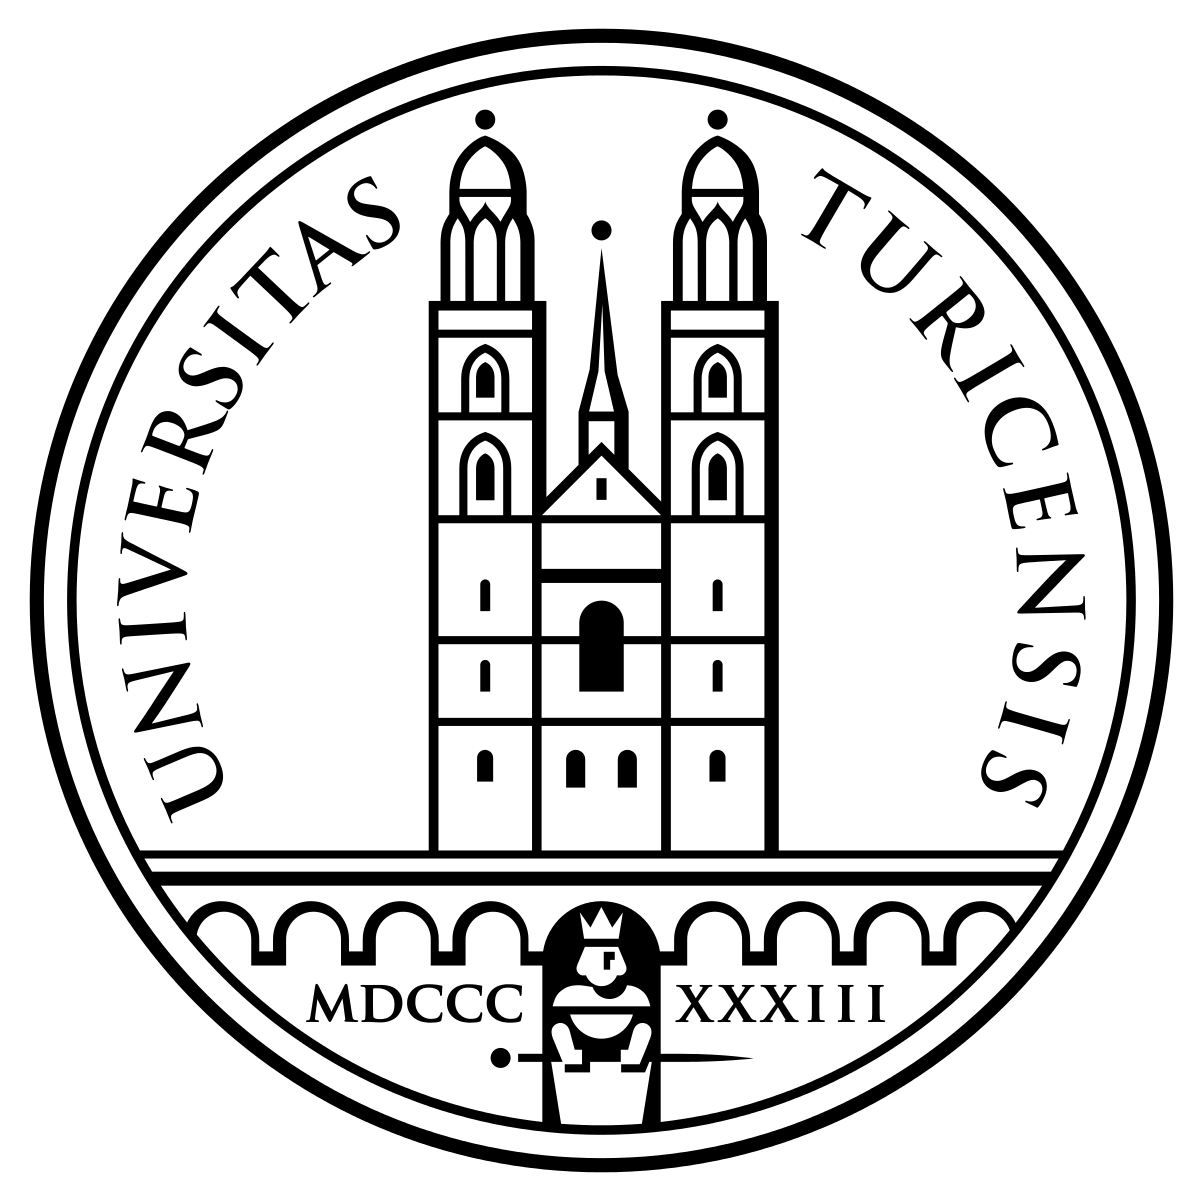
\includegraphics[width=0.5\textwidth]{frontespizio}
%\end{minipage}


\title[]{\textcolor{white}{\bfseries Spectral Lagrangian methods\\ (in particular for SW)}}

\author[Lorenzo Micalizzi] % (optional, for multiple authors)
{L.~Micalizzi\inst{1,2}, S.~Tokareva\inst{2}, M.~Ricchiuto\inst{3}, R.~Abgrall\inst{1}}

\institute[UZH] % (optional)
{
  \inst{1}%
  Institut f{\"u}r Mathematik,\\ 
  Universit{\"a}t Z{\"u}rich
  \and
  \inst{2}%
  Theoretical Division,\\
  Los Alamos National Laboratory
  \and
  \inst{3}%
  Team CARDAMOM,\\
  Inria Bordeaux sud-ouest
}

\date[Los Alamos] % (optional)
%{HONOM, April 2022}

%\begin{minipage}[c]{3truecm}
%\vspace{0.5cm}
%\includegraphics[width=2\textwidth]{HONOM2022_header}
%\end{minipage}





\logo{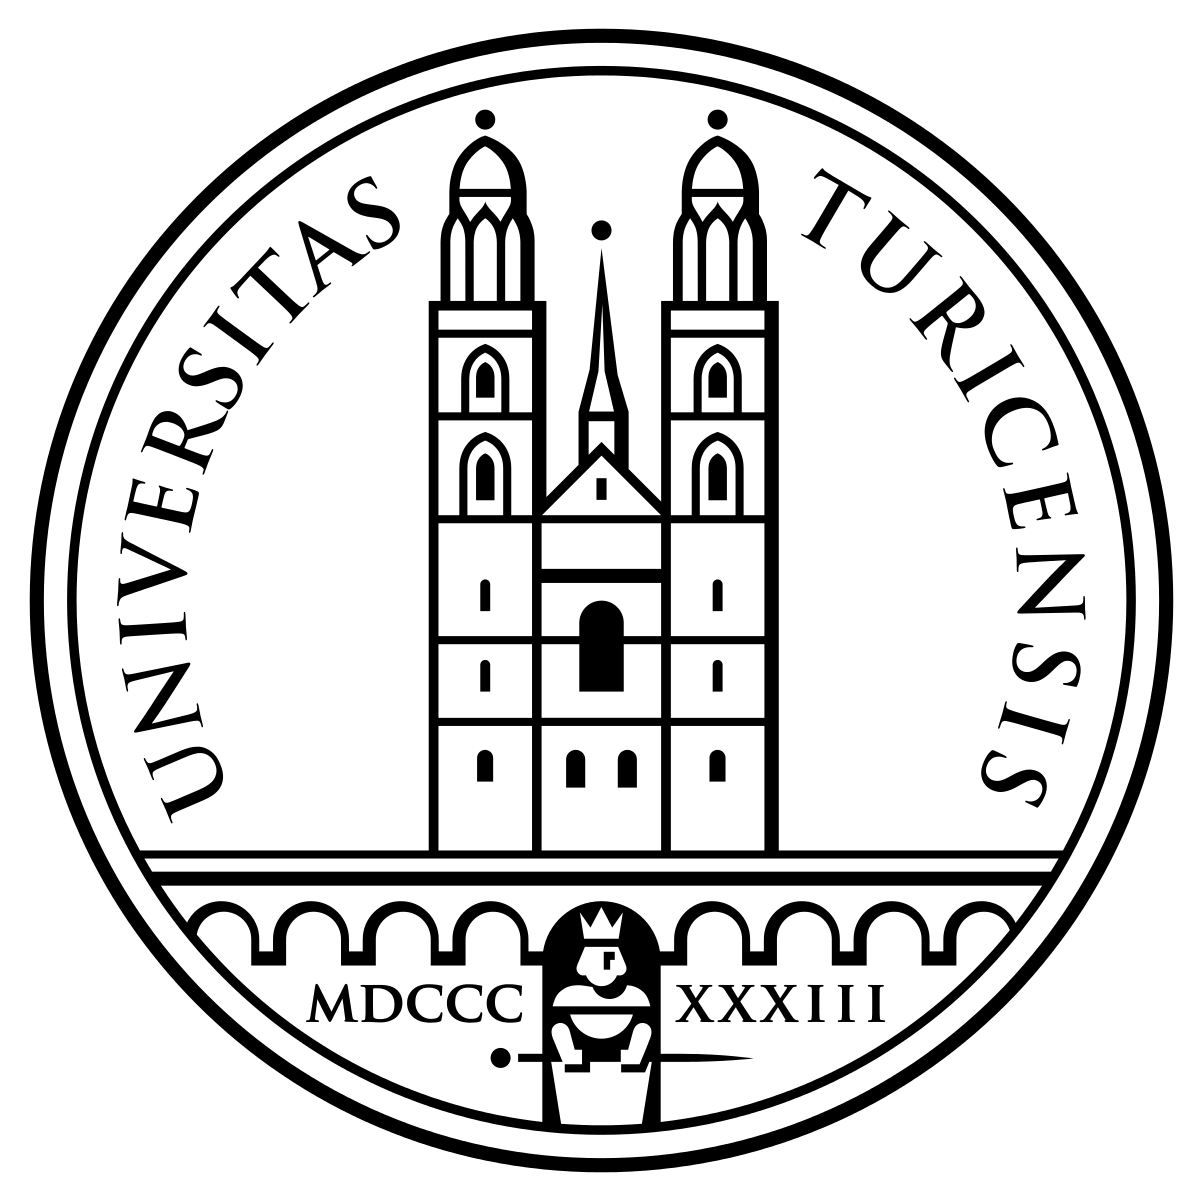
\includegraphics[height=1cm]{frontespizio.png}}

\begin{document}

\begin{frame}[plain]
\titlepage
\end{frame}



\begin{frame}[label=outline]
\frametitle{Outline}
\tableofcontents%[pausesections]

%\begin{itemize}
%
%\item Hyperbolic problems
%\item Numerical framework: Residual Distribution
%\item CIP techniques
%\item Numerical results 
%
%\end{itemize}

\end{frame}

\section{Governing equations}
\frame\sectionpage




\include{sslide}

\begin{frame}[label=SW]
\frametitle{Shallow water equations, Eulerian}
%We will mainly focus on

$$\frac{\partial}{\partial t}\uvec{u}+div_{\uvec{x}} \boldsymbol{F}(\uvec{u})=\boldsymbol{S}(\uvec{x},\uvec{u}), \quad (\uvec{x},t)\in \Omega \times [0,T]$$

    \begin{columns}

        \begin{column}{0.50\textwidth}
$$
\uvec{u}:=\begin{pmatrix}
H\\
H\uvec{v}\\
\end{pmatrix}$$
$$\uvec{F}(\uvec{u}):=\begin{pmatrix}
H\uvec{v}\\
H\uvec{v} \otimes \uvec{v}+\textcolor{SSCdarkgreen}{g}\frac{H^2}{2}\mathbb{I}
\end{pmatrix}$$
$$
\boldsymbol{S}(\uvec{x},\uvec{u}):=-\begin{pmatrix}
0\\
gH\nabla_{\uvec{x}} \textcolor{magenta}{B}(x)
\end{pmatrix}
$$

        \end{column}
        \begin{column}{0.50\textwidth}

	\begin{figure}
		\centering
		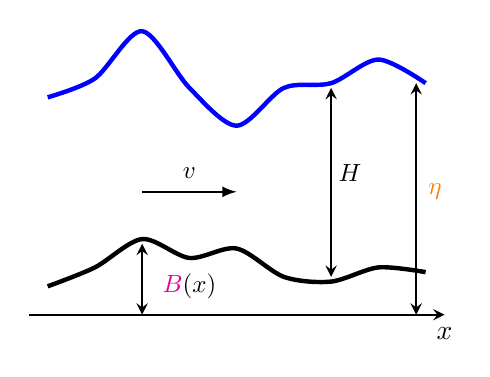
\begin{tikzpicture}[thick, scale=1.2]
			
			\draw [-stealth] (-0.2,-0.3) -- (4.2,-0.3);
			\node [black,scale=1] at (4.2,-0.5) {$x$};
			
			\draw [stealth-stealth] (1,-0.3) -- (1,0.45);
			\node [black,scale=0.9] at (1.5,0) {$\textcolor{magenta}{B}(x)$};
			\draw [stealth-stealth] (3,0.1) -- (3,2.1);
			\node [black,scale=0.9] at (3.2,1.2) {$H$};
			\draw [stealth-stealth] (3.9,-0.3) -- (3.9,2.15);
			\node [black,scale=0.9] at (4.1,1.0) {$\textcolor{orange}{\eta}$};
			
			\draw [-latex] (1,1) -- (2,1);
			\node [black,scale=0.9] at (1.5,1.2) {$v$};
			
			\draw [black,ultra thick] plot [smooth] coordinates {(0,0) (0.5,0.2) (1,0.5) (1.5,0.3) (2,0.4) (2.5,0.1) (3,0.05) (3.5,0.2) (4,0.15)};
			\draw [blue, ultra thick]  plot [smooth] coordinates {(0,2) (0.5,2.2) (1,2.7) (1.5,2.1) (2,1.7) (2.5,2.1) (3,2.15) (3.5,2.4) (4,2.15)};
			
		\end{tikzpicture}
		
	\end{figure}

        \end{column}
    \end{columns}


\centering
\vspace{1em}
$$\textcolor{orange}{\eta}:=H+B$$      

\end{frame}


\begin{frame}
\frametitle{Shallow water equations, simplification of Euler (with gravity)}

$$\frac{\partial}{\partial t}\uvec{u}+div_{\uvec{x}} \boldsymbol{F}(\uvec{u})=\boldsymbol{S}(\uvec{x},\uvec{u}), \quad (\uvec{x},t)\in \Omega \times [0,T]$$

    \begin{columns}

        \begin{column}{0.50\textwidth}
$$
\uvec{u}:=\begin{pmatrix}
H\\
H\uvec{v}\\
\end{pmatrix}$$
$$\uvec{F}(\uvec{u}):=\begin{pmatrix}
H\uvec{v}\\
H\uvec{v} \otimes \uvec{v}+\textcolor{SSCdarkgreen}{g}\frac{H^2}{2}\mathbb{I}
\end{pmatrix}$$
$$
\boldsymbol{S}(\uvec{x},\uvec{u}):=-\begin{pmatrix}
0\\
gH\nabla_{\uvec{x}} \textcolor{magenta}{B}(x)
\end{pmatrix}
$$

        \end{column}
        \begin{column}{0.50\textwidth}

\begin{align*}
H &\sim \rho\\
p &\sim \textcolor{SSCdarkgreen}{g}\frac{H^2}{2}\\
B(x) &\sim \phi(x)
\end{align*}


Neglecting the energy equation

        \end{column}
    \end{columns}



\end{frame}


\section{Scheme and motivation}
\frame\sectionpage


\begin{frame}
\frametitle{Shallow water equations, Lagrangian}

    \begin{columns}
        \begin{column}{0.50\textwidth}
\begin{align*}
\Omega_0  \ni \uvec{X} \longrightarrow & ~ \uvec{x}=\widetilde{\uvec{x}}(\uvec{X},t) \in \Omega_t\\
\widehat{\Omega}  \ni \uvec{\xi} \longrightarrow & ~\uvec{x}=\uvec{x}(\uvec{\xi},t) \in \Omega_t\\
& \uvec{X}=\uvec{x}(\uvec{\xi},0)
\end{align*}
        \end{column}
        \begin{column}{0.50\textwidth}

\begin{figure}
         \centering
         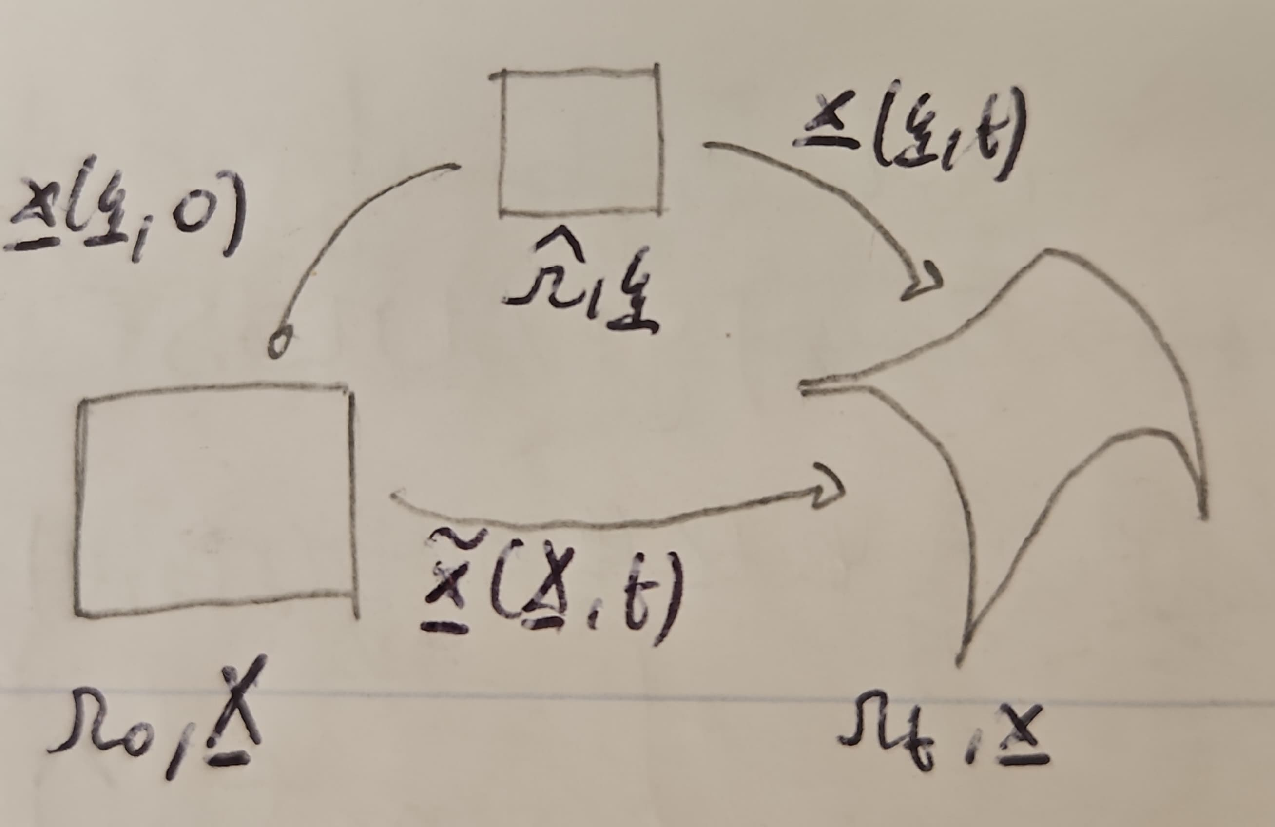
\includegraphics[width=0.9\textwidth]{figures/lagrangian_maps.pdf}
\end{figure}
        \end{column}
    \end{columns}
\end{frame}


\begin{frame}
\frametitle{Shallow water equations, Lagrangian}

\begin{itemize}

\item \textbf{Motion}
$$\frac{d}{dt}\uvec{x}(\uvec{\xi},t)=\uvec{v}(\uvec{x}(\uvec{\xi},t),t)$$

\item \textbf{Water height/density (SMC)} 
\begin{align*}
&H(\uvec{x}(\uvec{\xi},t),t)=\frac{\widehat{H}(\uvec{\xi})}{det \uvec{J}(\uvec{\xi},t)}, \quad \uvec{J}(\uvec{\xi},t)=\frac{\partial \uvec{x}}{\partial \uvec{\xi}}(\uvec{\xi},t)
\end{align*}


\item \textbf{Velocity} 
\begin{align*}
H(\uvec{x},t)\frac{d}{dt}\uvec{v}(\uvec{x},t)&=-\nabla_{\uvec{x}} p  -g H \nabla_{\uvec{x}}B\\
&=-\nabla_{\uvec{x}}\left(\frac{gH^2}{2}\right) -gH\nabla_{\uvec{x}}B
\end{align*}

$$\frac{d}{dt}\uvec{v}(\uvec{x},t)=-g\nabla_{\uvec{x}}(H+B)$$

\end{itemize}


\end{frame}




\begin{frame}
\frametitle{Shallow water equations, FEM discretization}

    \begin{columns}

        \begin{column}{0.50\textwidth}
\quad $\hphi_i\in \mathbb{P}_{M+1}$ continuous\\
\quad $\hpsi_i\in \mathbb{P}_{M}$ \quad discontinuous
        \end{column}
        \begin{column}{0.50\textwidth}
$$\varphi_i(\uvec{x}(\uvec{\xi},t),t)=\hphi_i(\uvec{\xi})$$
$$\psi_i(\uvec{x}(\uvec{\xi},t),t)=\hpsi_i(\uvec{\xi})$$
        \end{column}
    \end{columns}

\vspace{1cm}

    \begin{columns}

        \begin{column}{0.50\textwidth}
$$\uvec{x}_h(\uvec{\xi},t)=\sum_i\uvec{x}_i(t)\hphi_i(\uvec{\xi})$$
$$\uvec{v}_h(\uvec{\xi},t)=\sum_i\uvec{v}_i(t)\hphi_i(\uvec{\xi})$$
$$H_h(\uvec{\xi},t)=\sum_i H_i(t)\hpsi_i(\uvec{\xi})$$
        \end{column}
        \begin{column}{0.50\textwidth}
$$\uvec{v}_h(\uvec{x},t)=\sum_i\uvec{v}_i(t)\hphi_i(\uvec{\xi}(\uvec{x},t))$$
$$H_h(\uvec{x},t)=\sum_i H_i(t)\hpsi_i(\uvec{\xi}(\uvec{x},t))$$
        \end{column}
    \end{columns}


\end{frame}






\begin{frame}
\frametitle{Shallow water equations, discretized equations}

\begin{itemize}

\item \textbf{Motion}
$$\frac{d}{dt}\uvec{x}_i(t)=\uvec{v}_i(t)$$

\item \textbf{Water height/density (SMC) $\Rightarrow$ PP} 
\begin{align*}
&H_i(t)=\frac{\widehat{H}_i}{det \uvec{J}(\uvec{\xi}_i,t)}, \quad \uvec{J}(\uvec{\xi},t)=\frac{\partial \uvec{x}}{\partial \uvec{\xi}}(\uvec{\xi},t)
\end{align*}


\item \textbf{Velocity} 

\begin{align*}
\sum_{K \in K_i} & \sum_{\uvec{x}_j \in K} \Bigg(\int_K \varphi_i \varphi_j d \uvec{x}\Bigg) \frac{d}{dt}\uvec{v}_j(t)\\
&= -g \sum_{K \in K_i} \Bigg[ \int_K \varphi_i \nabla_{\uvec{x}}(H_h+B_h)  d\uvec{x}\Bigg] - \sum_{K \in K_i} \uvec{CT}_i^K -\uvec{ST}_i
\end{align*}

\end{itemize}


\end{frame}


\begin{frame}
\frametitle{Shallow water equations, discretized equations}


\begin{align*}
\sum_{K \in K_i} & \sum_{\uvec{x}_j \in K} \Bigg(\int_K \varphi_i \varphi_j d \uvec{x}\Bigg) \frac{d}{dt}\uvec{v}_j(t)\\
&= -g \sum_{K \in K_i} \Bigg[ \int_K \varphi_i \nabla_{\uvec{x}}(H_h+B_h)  d\uvec{x}\Bigg] - \sum_{K \in K_i} \uvec{CT}_i^K -\uvec{ST}_i
\end{align*}

\begin{align*}
\uvec{CT}_i^K=g\int_{\partial K} \varphi_i (\eta^*-\eta\vert_K) \uvec{\nu} d \uvec{\sigma}
\end{align*}



\begin{align*}
\uvec{ST}^{CIP}_i:=\sum_{f}\alpha_f  \biggl\llbracket \frac{\partial}{\partial x} \varphi_i\biggr\rrbracket  \biggl\llbracket \frac{\partial}{\partial x} v \biggr\rrbracket, \quad \uvec{ST}^{LxF}_i:= \sum_{K \in K_i} \alpha_K (\uvec{v}_i-\overline{\uvec{v}}_K)
\end{align*}

\centering

Last but not least an ODE integrator

\end{frame}


\begin{frame}
\frametitle{Problem: mass matrix}
\centering

\begin{align*}
\textcolor{red}{\sum_{K \in K_i}} & \textcolor{red}{\sum_{\uvec{x}_j \in K} \Bigg(\int_K \varphi_i \varphi_j d \uvec{x}\Bigg)} \frac{d}{dt}\uvec{v}_j(t)\\
&= -g \sum_{K \in K_i} \Bigg[ \int_K \varphi_i \nabla_{\uvec{x}}(H_h+B_h)  d\uvec{x}\Bigg] - \sum_{K \in K_i} \uvec{CT}_i^K -\uvec{ST}_i
\end{align*}


\begin{align*}
\textcolor{red}{\mathcal{M}}\frac{d}{dt}\uvec{v}=\uvec{r}
\end{align*}


\end{frame}



\begin{frame}
\frametitle{Solutions}

\begin{itemize}
\item LO mass lumping
\item DeC Remi\footnote{Abgrall, High order schemes for hyperbolic problems using globally continuous approximation and avoiding mass matrices, 2017} (problems for order 4 on)
\item \textcolor{red}{Spectral methods $\varphi_i \sim \uvec{x}_i$ ($1$D GLB, $2$D tensor product or Cubature)}
\end{itemize}

\end{frame}




\begin{frame}
\frametitle{Price to pay: time-dependent mass matrix}


\begin{align*}
\int_{K(t)} \varphi_i(\uvec{x},t)\varphi_j(\uvec{x},t)d\uvec{x}&=\int_{\widehat{K}} \hphi_i(\uvec{\xi})\hphi_j(\uvec{\xi}) det \uvec{J}(\uvec{\xi},t) d\uvec{\xi}\\
&\approx \delta_{i,j}\widehat{\omega}_i \textcolor{red}{det \uvec{J}(\uvec{\xi}_i,t)}
\end{align*}


\begin{align*}
\int_{K(t)}H_h(\uvec{x},t) \varphi_i(\uvec{x},t)\varphi_j(\uvec{x},t)d\uvec{x}&=\int_{\widehat{K}}H_h(\uvec{\xi},t) \hphi_i(\uvec{\xi})\hphi_j(\uvec{\xi}) det \uvec{J}(\uvec{\xi},t) d\uvec{\xi}\\
&\approx \delta_{i,j}\widehat{\omega}_i \textcolor{red}{ H_h(\uvec{\xi}_i,t) det \uvec{J}(\uvec{\xi}_i,t)}
\end{align*}

\centering 
However, only a point evaluation

\end{frame}



\begin{frame}
\frametitle{Advantages}

\begin{align*}
\frac{d}{dt}\uvec{x}=\uvec{v}, \quad \frac{d}{dt}\uvec{v}=\uvec{r}, \quad \text{SMC}
\end{align*}


\begin{itemize}

\item Truly arbitrary high order (no problems as for Bernstein and $\beta$-limiting)

\item Extendible to Euler

\item Extendible to multi-D (quads, PGL, tensor products, Cubature)

\item Whatever time integration method.

\end{itemize}

\end{frame}


\section{Numerics}
\frame\sectionpage


\begin{frame}
\frametitle{Numerics, Sod (Sorry for low quality)}


\begin{figure}
     \centering
     \begin{subfigure}[b]{0.3\textwidth}
         \centering
         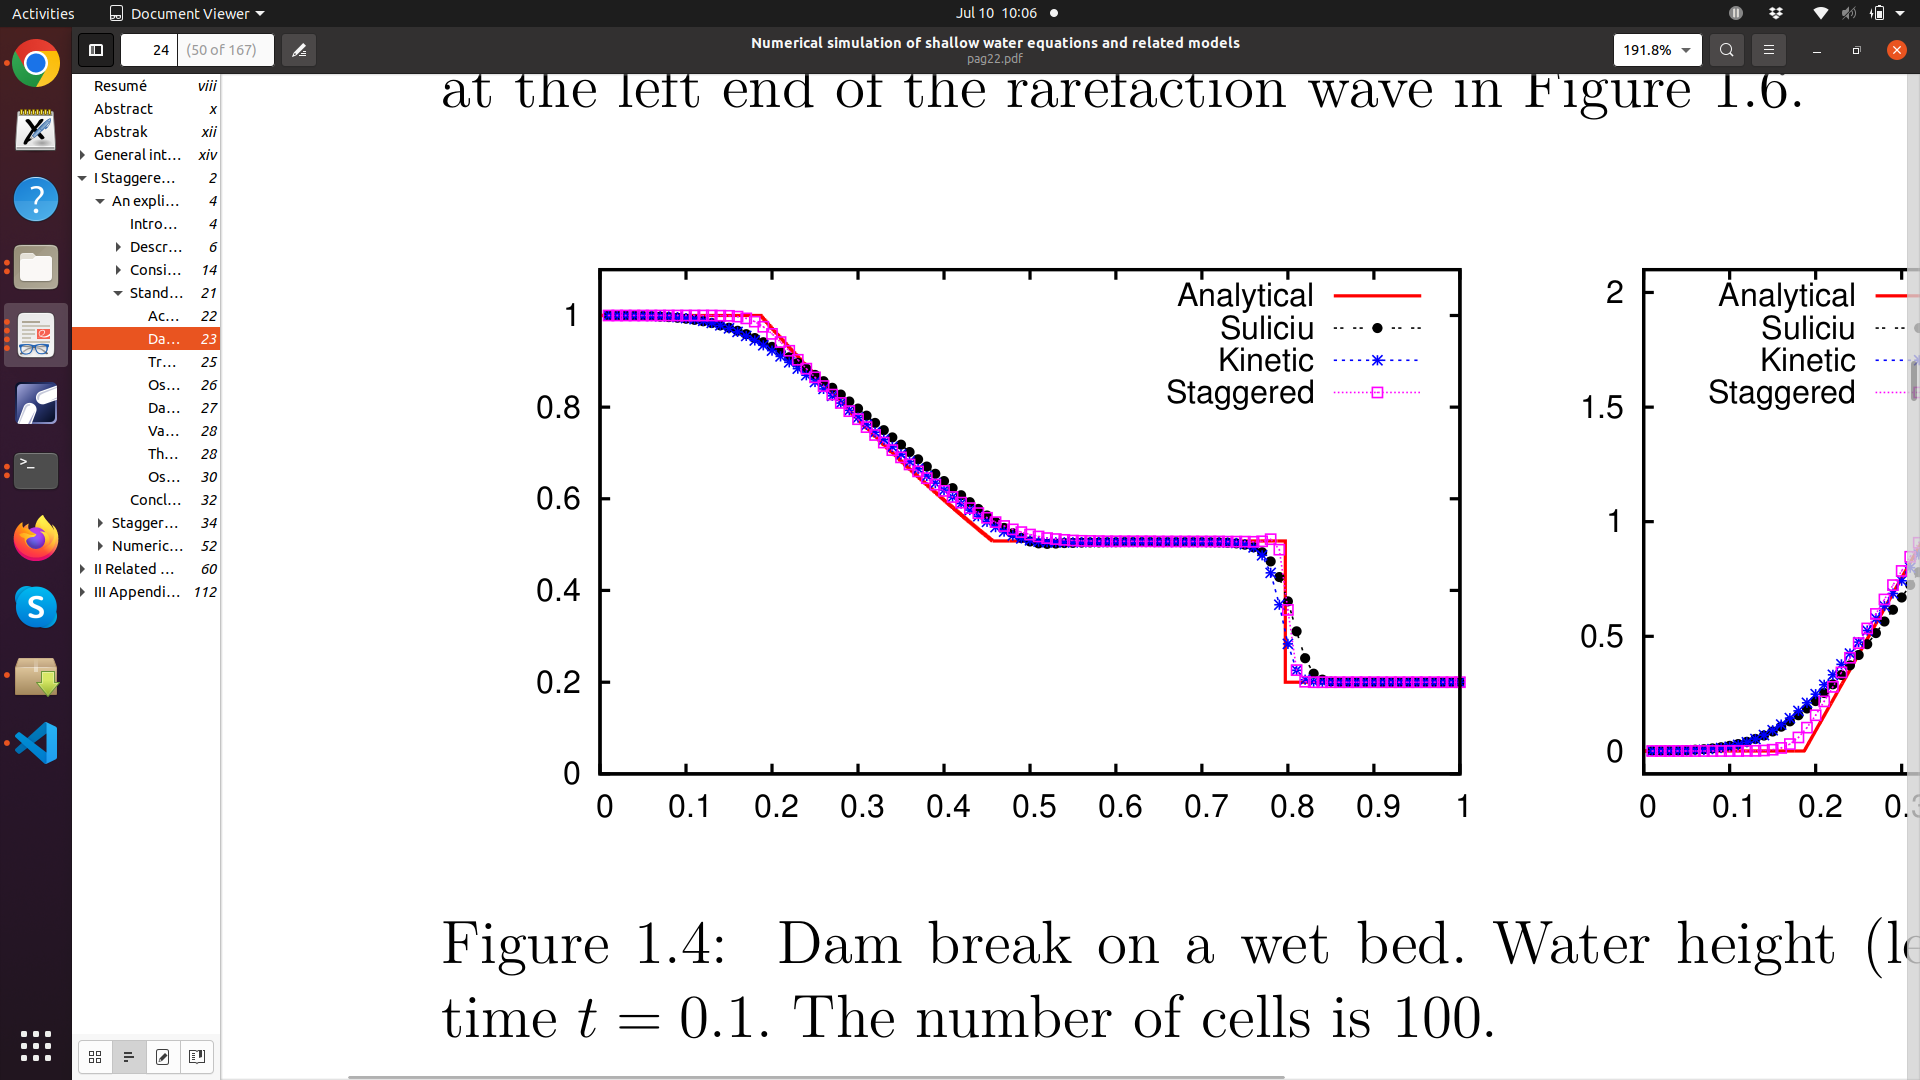
\includegraphics[width=\textwidth]{figures/sod/reference.png}
     \end{subfigure}
     \begin{subfigure}[b]{0.8\textwidth}
         \centering
         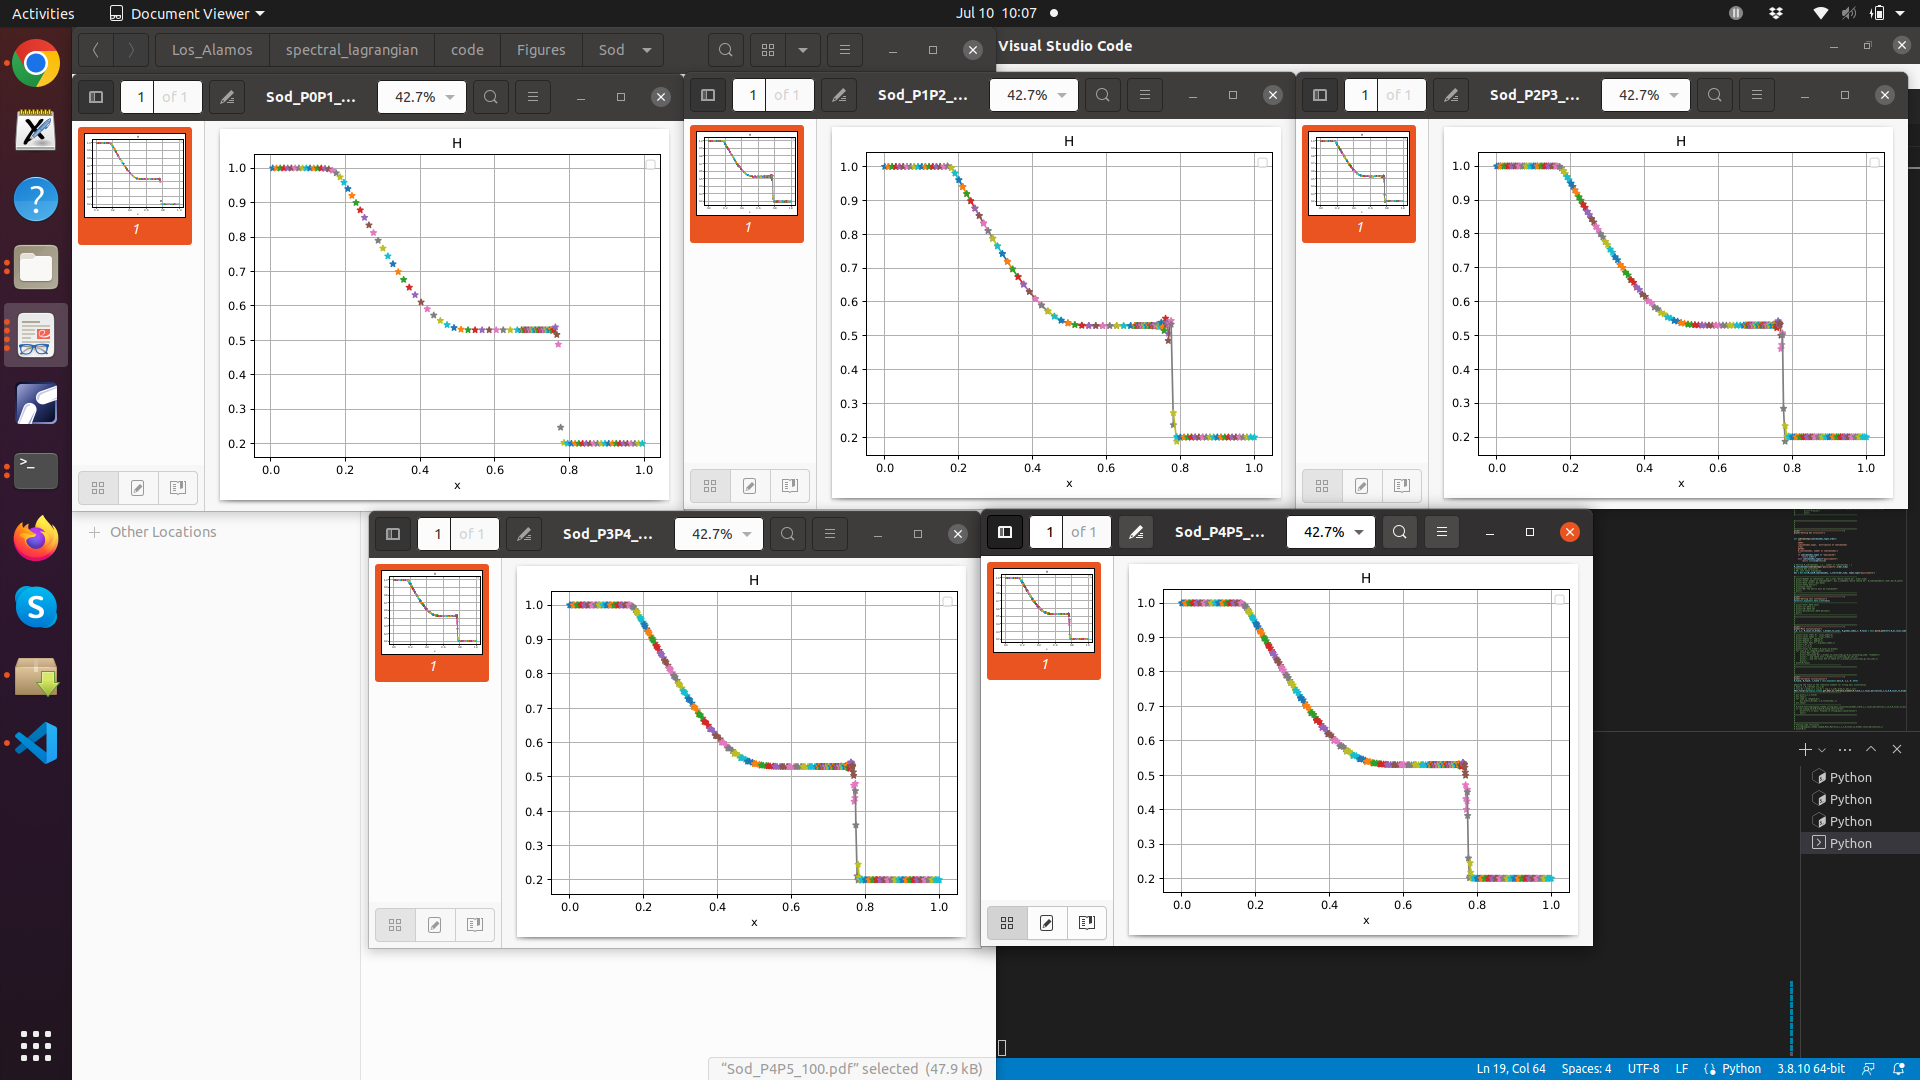
\includegraphics[width=\textwidth]{figures/sod/my_results.png}
     \end{subfigure}
\end{figure}


\end{frame}


\begin{frame}
\frametitle{Numerics, Convergence\footnote{Mantri, Oeffner, Ricchiuto, Fully well balanced entropy controlled DGSEM, 2022} ($2p$)}

\begin{align}
\begin{cases}
H=2+cos(2\pi x)\\
v=1
\end{cases}
\end{align}



\begin{figure}
     \centering
         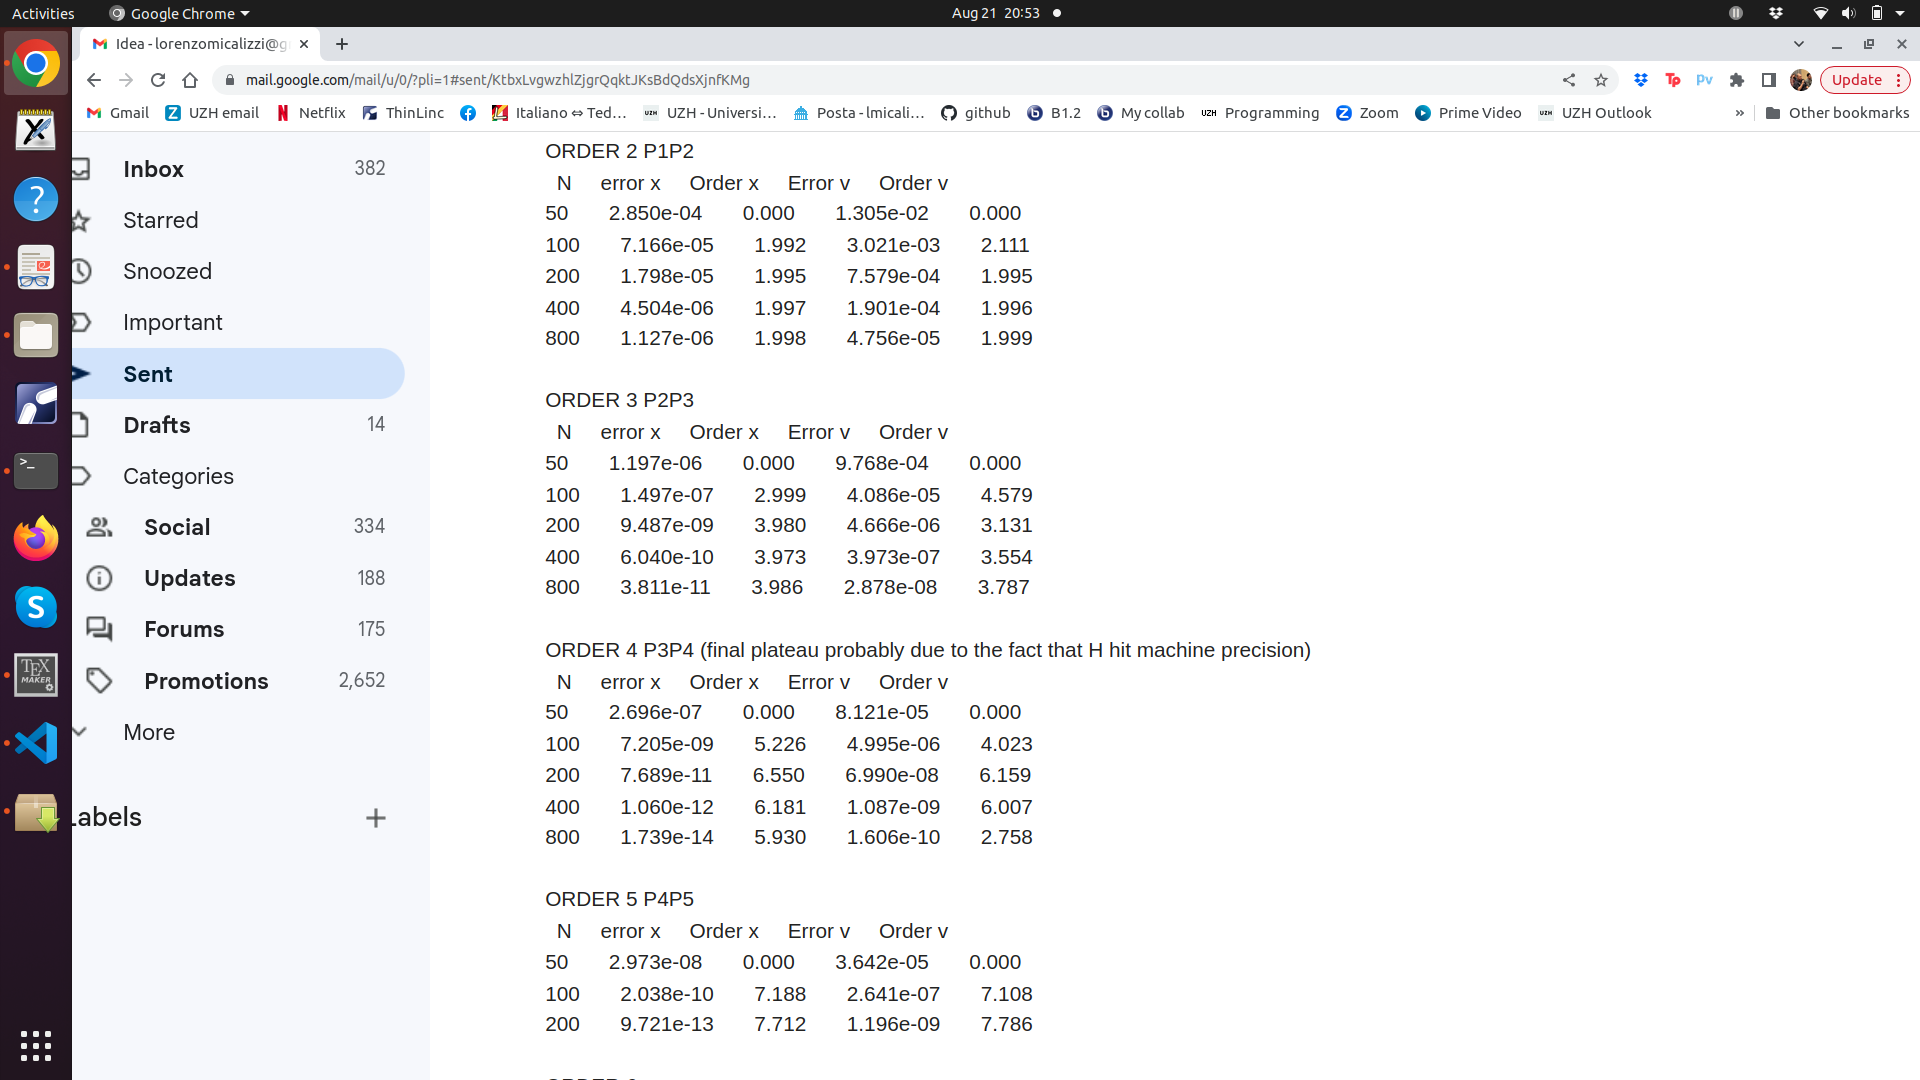
\includegraphics[width=0.8\textwidth]{figures/smooth_periodic/conv.png}
\end{figure}


\end{frame}


\begin{frame}
\frametitle{Numerics, well-balancing}

In particular (in Eulerian) $\textcolor{red}{\frac{\partial}{\partial t}\uvec{u}\equiv 0 ~ \Leftrightarrow ~ \frac{\partial}{\partial x}\boldsymbol{F}(\uvec{u})=\boldsymbol{S}(x,\uvec{u}) }$)


\begin{itemize}
\item Refine a lot the mesh $\Rightarrow$ Longer computational time
\item Well-balancing 
\end{itemize}



\scalebox{0.8}{\begin{minipage}[t]{1.2\textwidth}
	\begin{beamercolorbox}[sep=0.5em,wd=\textwidth]{blockcolor1} 
\begin{columns}
	\begin{column}{0.4\textwidth}
$$
\uvec{u}_{eq}:=\begin{pmatrix}
\eta-B\\
0
\end{pmatrix}$$	
$$\eta=H+B\equiv const$$ 
	\end{column}
	\begin{column}{0.40\textwidth}
\begin{figure}[hp] \centering{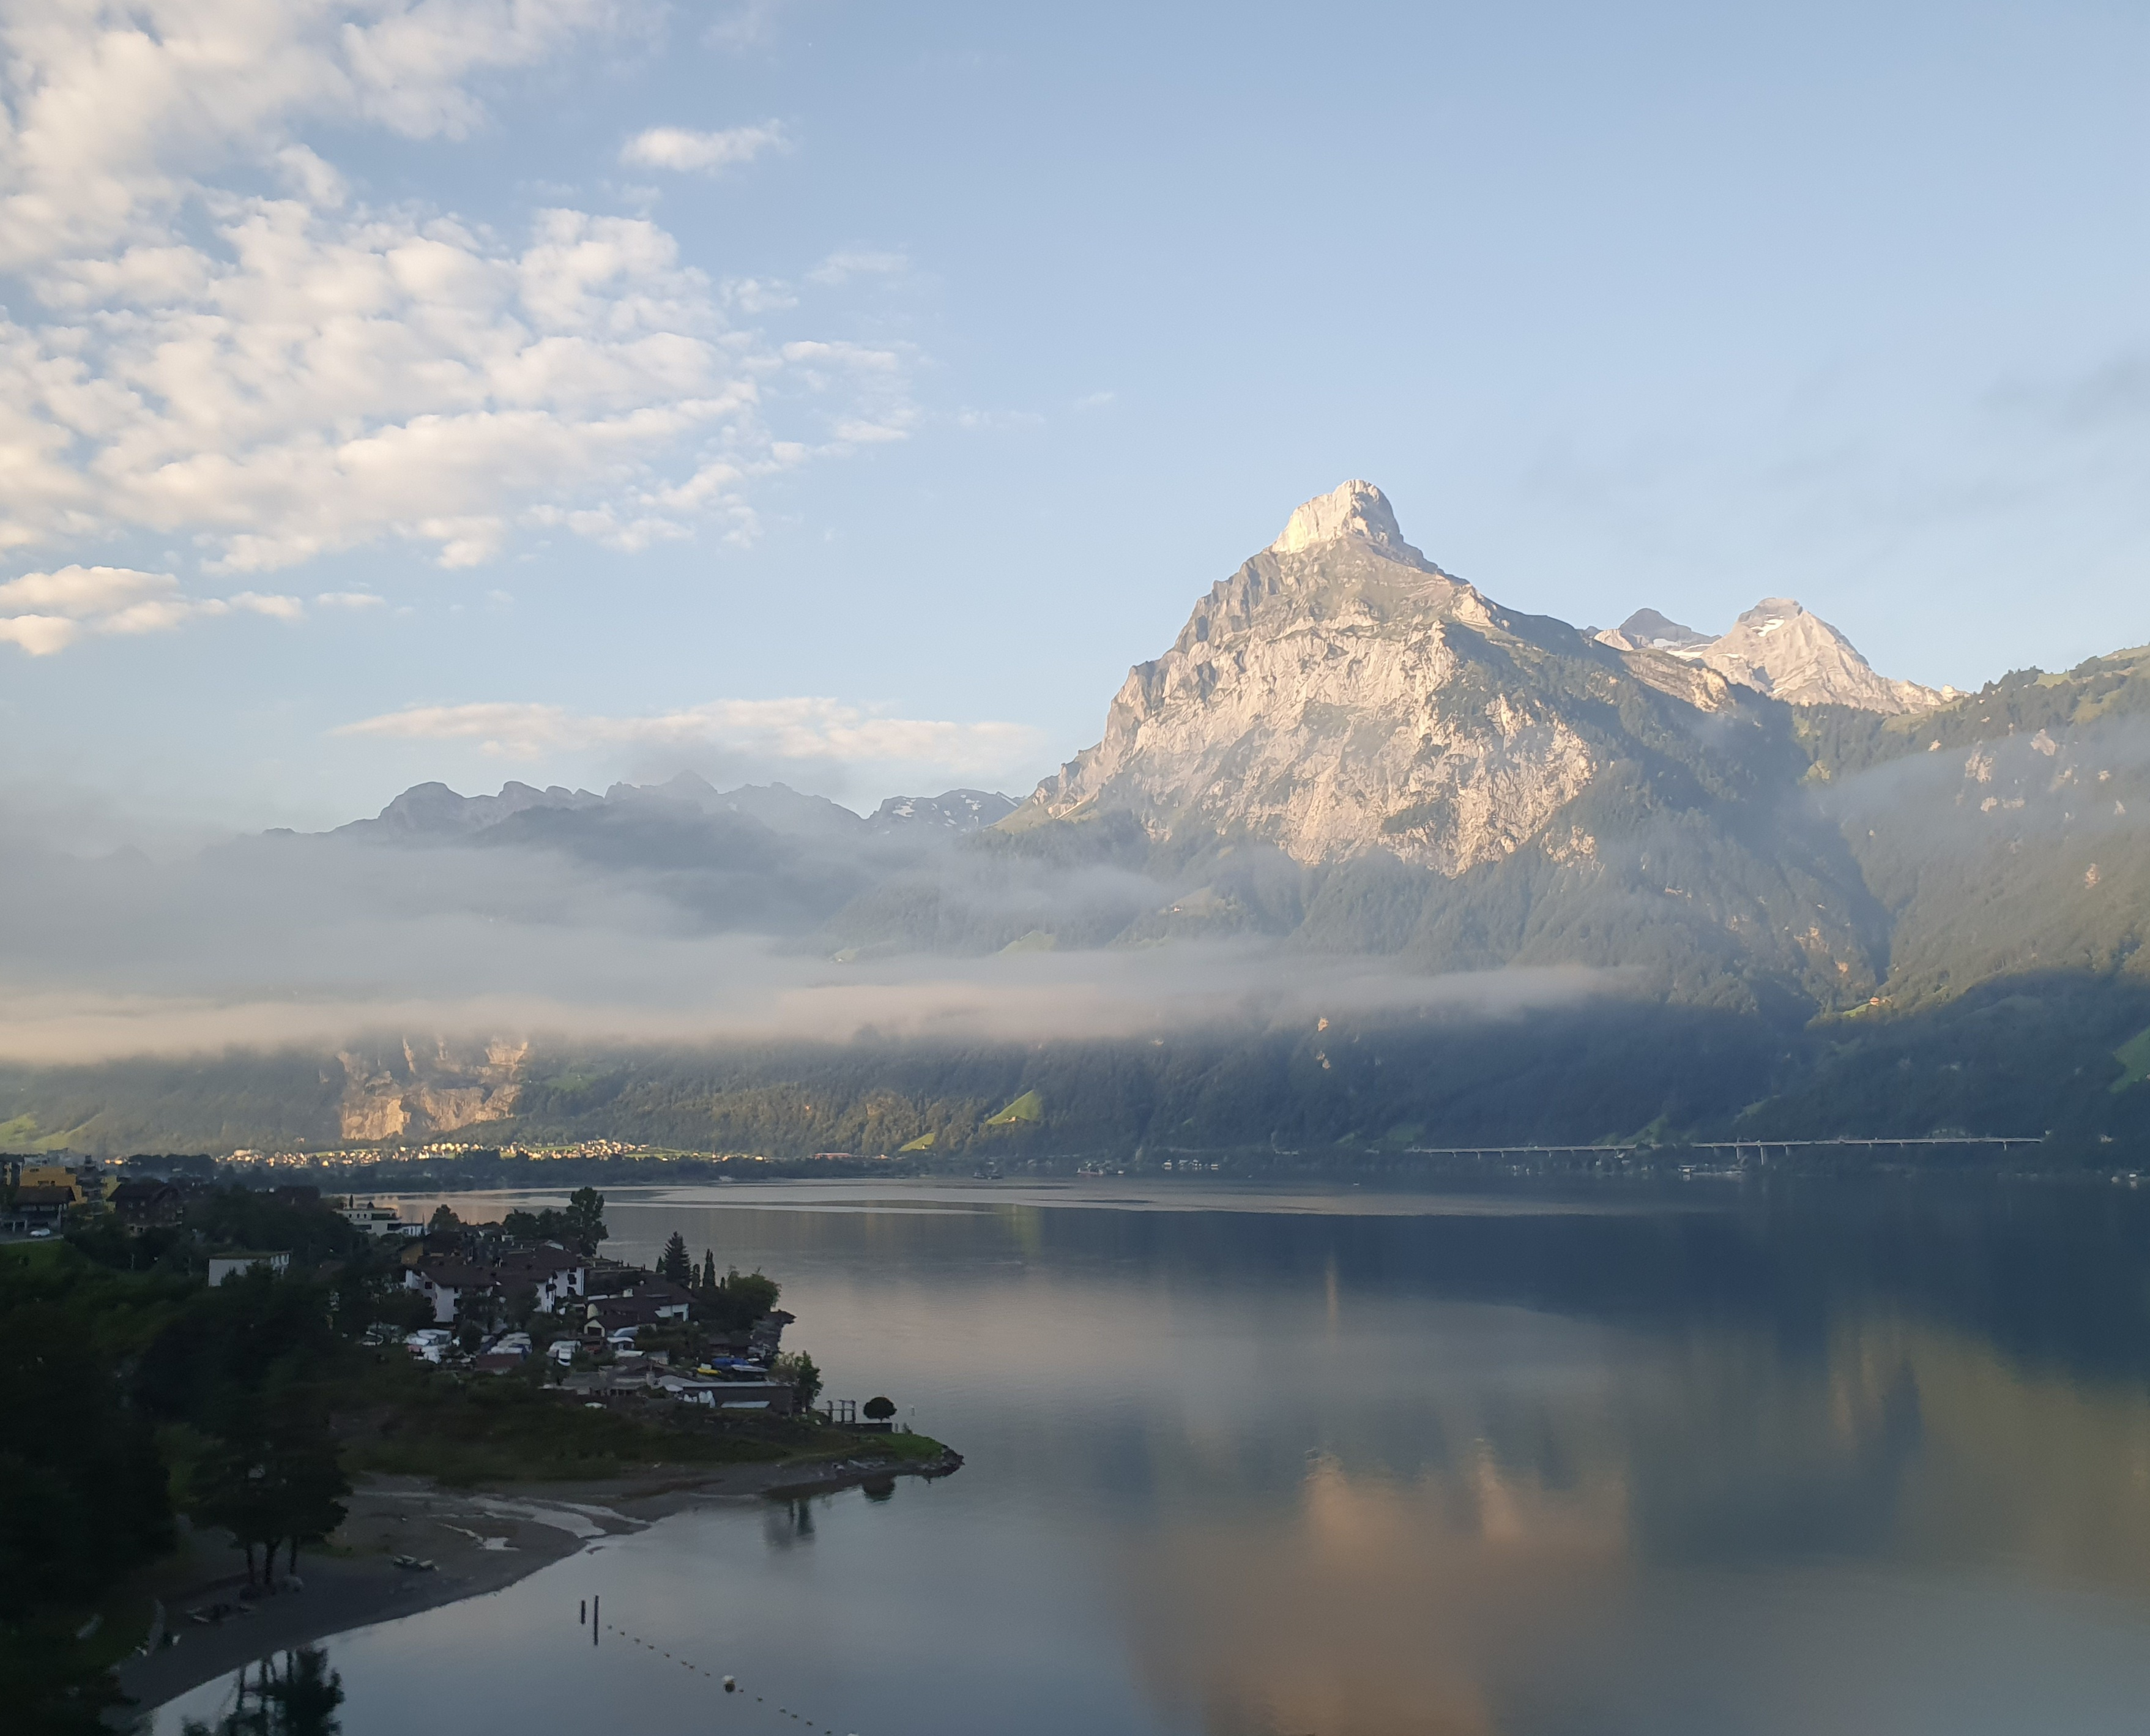
\includegraphics[scale=0.05]{lakezurich.jpg}}
\caption{Lake of Z{\"u}rich at rest}
\label{lakezurich}
\end{figure}

    \end{column}
\end{columns} 
\end{beamercolorbox}
\end{minipage}}



\end{frame}



\begin{frame}
\frametitle{Numerics, well-balancing}
Non-smooth bathymetry, only $C^0$

$$\eta(x)=\begin{cases}
\eta_{eq}+A\exp{\left(1-\frac{1}{1-\left(\frac{x-6}{0.5}\right)^2}\right)} & 5.5<x<6.5\\
\eta_{eq} & otherwise
\end{cases}$$
with $A=5\cdot 10^{-5}$.

\begin{figure}
         \centering
         \includegraphics[width=0.45\textwidth]{figures/lakeatrest/alb_latr_pert_IC.pdf}
         \caption{Perturbation amplified by $1000$}
\end{figure}


\end{frame}

\begin{frame}
\frametitle{Numerics, well-balancing}


\begin{figure}
         \centering
         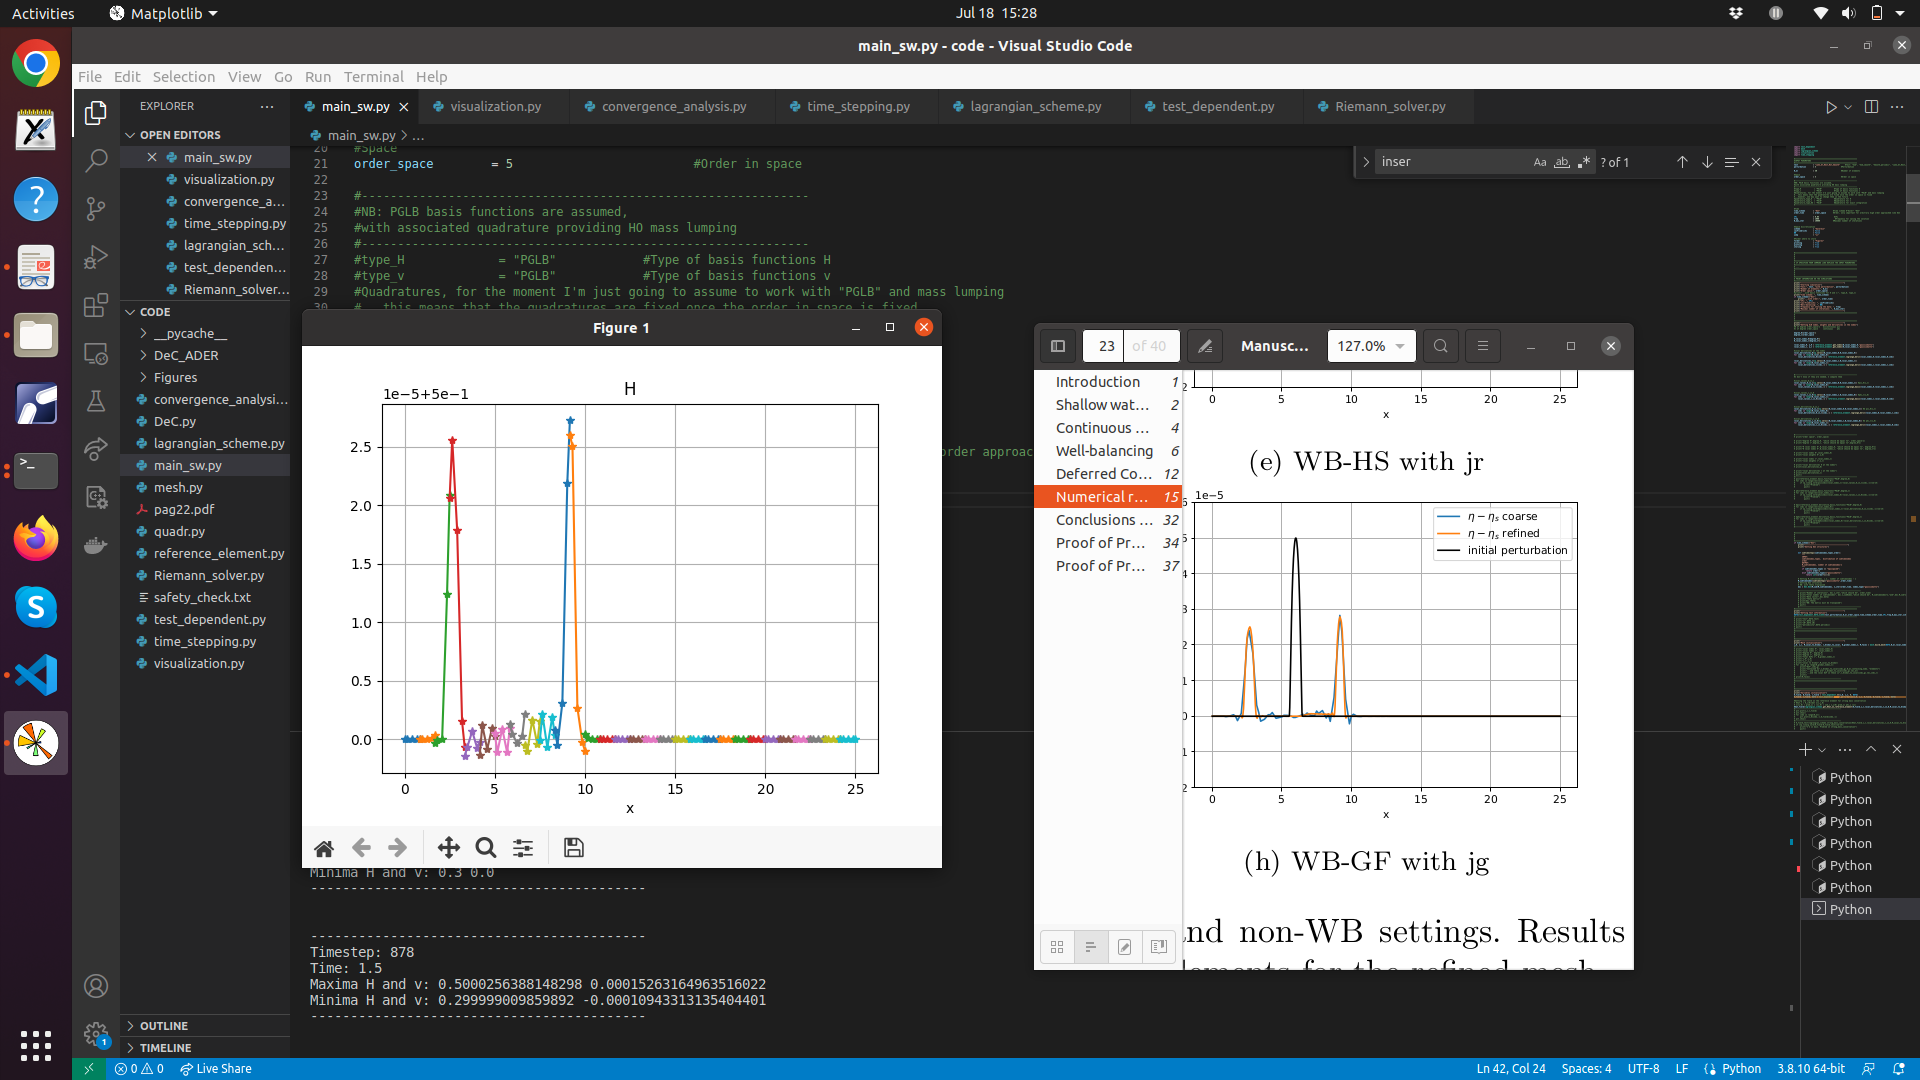
\includegraphics[width=1.2\textwidth]{figures/lakeatrest/perturbation.png}
\end{figure}


\end{frame}

\section{Continuous FEM}
\frame\sectionpage




\begin{frame}
\frametitle{Continuous FEM}
\scalebox{0.9}{\begin{minipage}[t]{1.2\textwidth}
	\begin{beamercolorbox}[sep=0.5em,wd=\textwidth]{blockcolor1} 
\begin{itemize}
\item A tessellation $\tess=\left\lbrace  K \right\rbrace $ of $\Omega$;
\visible<2->{\item The space $V_h$ of continuous piecewise polynomial functions;}
\visible<3->{\item a basis $\lbrace \varphi_i \rbrace_{i=1,\dots,I}$ of $V_h$ (B$n$, P$n$, PGL$n$);}
\visible<4->{\item We look for $\uvec{u}_h(x,t):=\sum_{j=1}^I\uvec{c}_j(t)\varphi_j(x)$ s.t.}


\end{itemize}
	\centering

\visible<4->{
\begin{align*}
\int_\Omega \biggl( \frac{\partial}{\partial t}\uvec{u}_h + \textcolor{red}{\biggl[\frac{\partial}{\partial x}   \boldsymbol{F}(\uvec{u}_h) } & \textcolor{red}{-\boldsymbol{S}(x,\uvec{u}_h) \biggr]_h} \biggr) \varphi_i(x) +\textcolor{blue}{\textbf{ST}_i(\uvec{u}_h)} =\uvec{0}  \quad \forall i\\
\visible<5->{   & \Downarrow ~  & \\
\massmatrix \frac{d}{dt}\uvec{c} &(t) =  \uvec{H}(\uvec{c}(t)) }\\\\\\
\visible<6->{\uvec{u}_{eq}:=\begin{pmatrix}
\eta-B\\
0
\end{pmatrix}, & \quad \eta=H+B\equiv const}
\end{align*}}

\end{beamercolorbox}
\end{minipage}} 



\end{frame}







\section{Well-balancing}
\frame\sectionpage





\subsection{Spatial part}
\frame\subsectionpage


\begin{frame}
\frametitle{Spatial part}


\begin{align*}
&\textcolor{red}{\biggl[\frac{\partial}{\partial x}   \boldsymbol{F}(\uvec{u}_h) }  \textcolor{red}{-\boldsymbol{S}(x,\uvec{u}_h) \biggr]_h}=\frac{\partial}{\partial x}   \textcolor{magenta}{\boldsymbol{F}_h}(x)-\textcolor{SSCdarkgreen}{\boldsymbol{S}_h}(x)\visible<2->{\neq 0~\text{for~lake~at~rest}}\\
&\textcolor{magenta}{\boldsymbol{F}_h}(x)=\sum_{j}\uvec{F}_j\varphi_j(x), \quad \textcolor{SSCdarkgreen}{\boldsymbol{S}_h}(x) = \sum_{j}\uvec{S}_j \varphi_j(x)
\end{align*}
%
\visible<3->{Special WB discretization\only<3->{\footnote{Ricchiuto and Bollermann. Stabilized residual distribution for shallow water simulations, 2009}}
\only<3>{
\begin{align*}
\textcolor{red}{\biggl[\frac{\partial}{\partial x}   \boldsymbol{F}(\uvec{u}_h) } \textcolor{red}{-\boldsymbol{S}(x,\uvec{u}_h) \biggr]_h}&=\left[\frac{\partial}{\partial x} \begin{pmatrix}
Hv\\
Hv^2 +g\textcolor{orange}{\frac{H^2}{2}}
\end{pmatrix}+\begin{pmatrix}
0\\
g\textcolor{orange}{H\frac{\partial}{\partial x} B}
\end{pmatrix} \right]_h\\
&=\frac{\partial}{\partial x}\left[\begin{pmatrix}
Hv\\
Hv^2
\end{pmatrix}\right]_h +\begin{pmatrix}
0\\
g \textcolor{orange}{H_h \frac{\partial}{\partial x}}\Bigg( \textcolor{orange}{H_h} + \textcolor{orange}{B_h} \Bigg)
\end{pmatrix}
\end{align*}}
\only<4->{
\begin{align*}
\textcolor{red}{\biggl[\frac{\partial}{\partial x}   \boldsymbol{F}(\uvec{u}_h) } \textcolor{red}{-\boldsymbol{S}(x,\uvec{u}_h) \biggr]_h}&=\left[\frac{\partial}{\partial x} \begin{pmatrix}
Hv\\
Hv^2 +g\textcolor{orange}{\frac{H^2}{2}}
\end{pmatrix}+\begin{pmatrix}
0\\
g\textcolor{orange}{H\frac{\partial}{\partial x} B}
\end{pmatrix} \right]_h\\
&=\frac{\partial}{\partial x}\left[\begin{pmatrix}
Hv\\
Hv^2
\end{pmatrix}\right]_h +\begin{pmatrix}
0\\
g \textcolor{orange}{H_h \frac{\partial}{\partial x}}\Bigg( \textcolor{red}{H_h} + \textcolor{red}{B_h} \Bigg)
\end{pmatrix}=\uvec{0}
\end{align*}}
}





\end{frame}













\subsection{Stabilization, continuous interior penalty}
\frame\subsectionpage
\begin{frame}
\frametitle{Stabilization part}

\begin{align*}
\int_\Omega \varphi_i(x) \frac{\partial}{\partial t}\uvec{u}_h d \uvec{x}+ \int_\Omega \varphi_i(x) & \textcolor{red}{\biggl[\frac{\partial}{\partial x}   \boldsymbol{F}(\uvec{u}_h) } \textcolor{red}{-\boldsymbol{S}(x,\uvec{u}_h) \biggr]_h} +\textcolor{blue}{\textbf{ST}_i(\uapp)}=\uvec{0} \quad \forall i
\end{align*}


\vspace{0.2em}

\visible<2->{CIP\only<2->{\footnote{J. Douglas Jr and T. Dupont Interior Penalty Procedures for Elliptic and Parabolic Galerkin Methods, 1976}} stabilization terms (\textbf{jump c})
\begin{align*}
\textbf{ST}_i(\uapp) &:=\sum_{f}\alpha_f \int_f [\![ \nabla_{\uvec{x}} \varphi_i]\!]  [\![ \nabla_{\uvec{x}} \uvec{u}_h ]\!] d\sigma \\
\visible<2->{&=\sum_{f}\alpha_f  \biggl\llbracket \frac{\partial}{\partial x} \varphi_i\biggr\rrbracket  \biggl\llbracket \frac{\partial}{\partial x} \uvec{u}_h \biggr\rrbracket }\\
%%%%%%\only<2>{&=\sum_{f}\alpha_f  \biggl\llbracket \frac{\partial}{\partial x} \varphi_i\biggr\rrbracket  \biggl\llbracket \frac{\partial}{\partial x} \begin{pmatrix}
%%%%%%H_h \\
%%%%%%(H v)_h
%%%%%%\end{pmatrix} \biggr\rrbracket}
\only<3->{&=\sum_{f}\alpha_f  \biggl\llbracket \frac{\partial}{\partial x} \varphi_i\biggr\rrbracket  \biggl\llbracket \frac{\partial}{\partial x} \begin{pmatrix}
\textcolor{magenta}{H_h} \\
(H v)_h
\end{pmatrix} \biggr\rrbracket}\visible<3->{\neq \uvec{0}}
\end{align*}
}

\end{frame}

\begin{frame}
\frametitle{Stabilization part, novel well-balanced jumps}

\begin{itemize}
\visible<1->{\item \textbf{jump t} (total height)

$$\textbf{ST}_i(\uapp):=\sum_{f}\alpha_f  \biggl\llbracket \frac{\partial}{\partial x} \varphi_i\biggr\rrbracket  \biggl\llbracket \frac{\partial}{\partial x} \begin{pmatrix}
\eta \\
H v
\end{pmatrix} \biggr\rrbracket$$
}


\visible<2->{\item \textbf{jump e} (entropy variables)

$$\textbf{ST}_i(\uapp):=\sum_{f}\alpha_f  \biggl\llbracket \frac{\partial}{\partial x} \varphi_i\biggr\rrbracket \frac{\partial \uvec{u}}{\partial \uvec{w}}  \biggl\llbracket \frac{\partial}{\partial x} \uvec{w} \biggr\rrbracket, \quad \uvec{w}:=\begin{pmatrix}
g\eta-\frac{v^2}{2}\\
v
\end{pmatrix}$$
}

\visible<3->{\item \textcolor{red}{\textbf{jump r} (residual)}

$$\textbf{ST}_i(\uapp):=\sum_{f}\alpha_f  \biggl\llbracket \boldsymbol{J} \frac{\partial}{\partial x} \varphi_i\biggr\rrbracket \vert \boldsymbol{J} \vert^{-1}  \biggl\llbracket \textcolor{red}{ \uvec{J}\frac{\partial}{\partial x} \uvec{u}-\uvec{S}} \biggr\rrbracket, \quad \uvec{J}:=\frac{\partial \uvec{F}}{\partial \uvec{u}}$$
}




\end{itemize}



\end{frame}






\section{Numerical results}
\frame\sectionpage

\begin{frame}
\frametitle{Well-balancing}

\scalebox{0.8}{\begin{minipage}[t]{1.2\textwidth}
	\begin{beamercolorbox}[sep=0.5em,wd=\textwidth]{blockcolor1} 
\begin{columns}
	\begin{column}{0.4\textwidth}
\begin{figure}
         \centering
         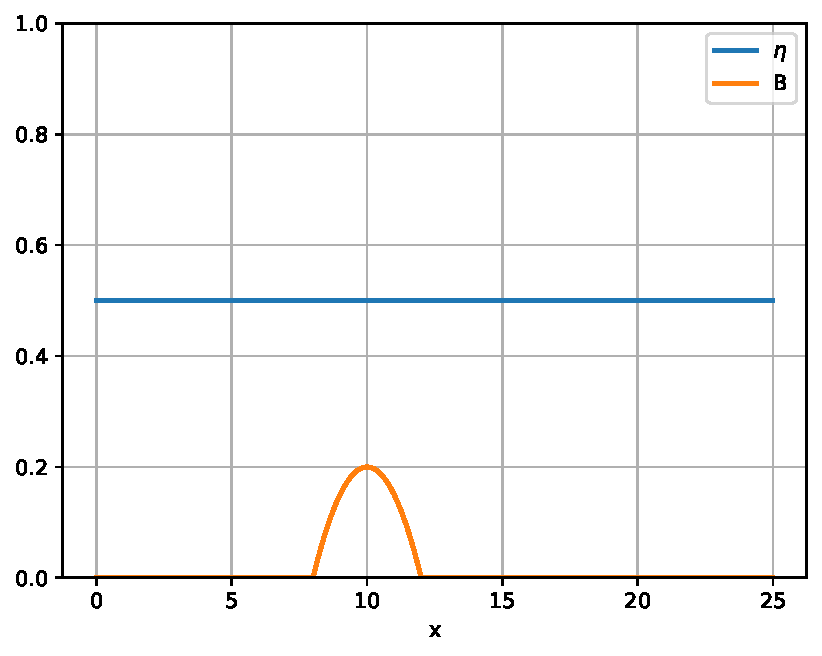
\includegraphics[width=0.9\textwidth]{alb_LAKEATREST.pdf}
\end{figure}
	\end{column}
	\begin{column}{0.50\textwidth}

\begin{table}
\centering
 \begin{tabular}{||c c c||} 
 \hline
  Framework   & $L^1$ error $H$  & $L^1$ error $Hv$ \\
  \hline 
 WB-HS jc  & 3.007E-004 &  5.963E-004 \\
  \hline 
 WB-HS jt  & 9.403E-013 &  4.418E-012 \\
  \hline
 WB-HS je  & 9.396E-013 &  4.415E-012 \\
  \hline  
 WB-HS jr  & 9.409E-013 &  4.415E-012 \\
  \hline  
\end{tabular}
\caption{\label{tabwblatr} PGL4 with $100$ elements at $T_f=10$}
%with CFL=0.05
\end{table}
Same with P$n$ and B$n$

    \end{column}
\end{columns} 
\end{beamercolorbox}
\end{minipage}}

\end{frame}



\begin{frame}
\frametitle{Small perturbation of lake at rest}
Same domain, non-smooth bathymetry, only $C^0$

$$\eta(x)=\begin{cases}
\eta_{eq}+A\exp{\left(1-\frac{1}{1-\left(\frac{x-6}{0.5}\right)^2}\right)} & 5.5<x<6.5\\
\eta_{eq} & otherwise
\end{cases}$$
with $A=5\cdot 10^{-5}$.

\begin{figure}
         \centering
         \includegraphics[width=0.45\textwidth]{alb_latr_pert_IC.pdf}
         \caption{Perturbation amplified by $1000$}
\end{figure}


\end{frame}








\begin{frame}
\frametitle{Small perturbation of lake at rest}
\centering
{\small PGL4; coarse: $30$ elements; refined: $128$ elements}
\begin{figure}
     \centering
     \begin{subfigure}[b]{0.3\textwidth}
         \centering
         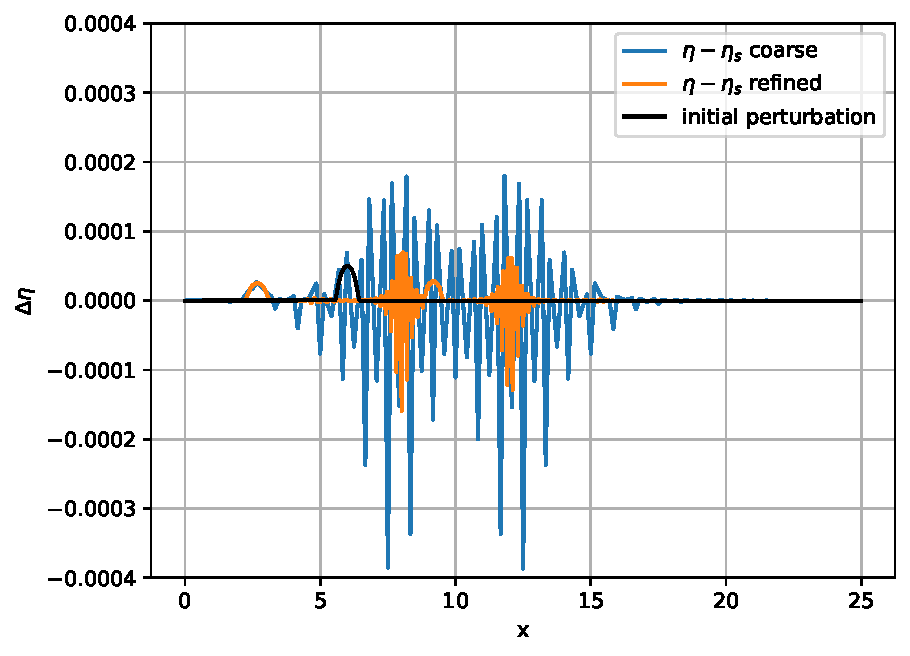
\includegraphics[width=\textwidth]{alb_latr_WBp3s14jc.pdf}
         \caption{Jump c}
     \end{subfigure}
     \begin{subfigure}[b]{0.3\textwidth}
         \centering
         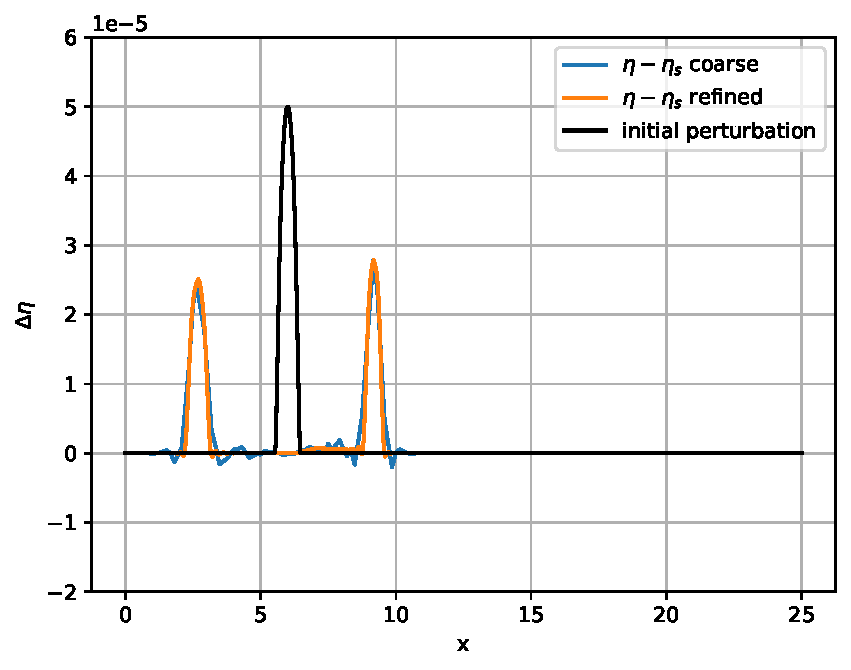
\includegraphics[width=\textwidth]{alb_latr_WBp3s14jt.pdf}
         \caption{Jump t}
     \end{subfigure}
     \vskip\baselineskip
     \begin{subfigure}[b]{0.3\textwidth}
         \centering
         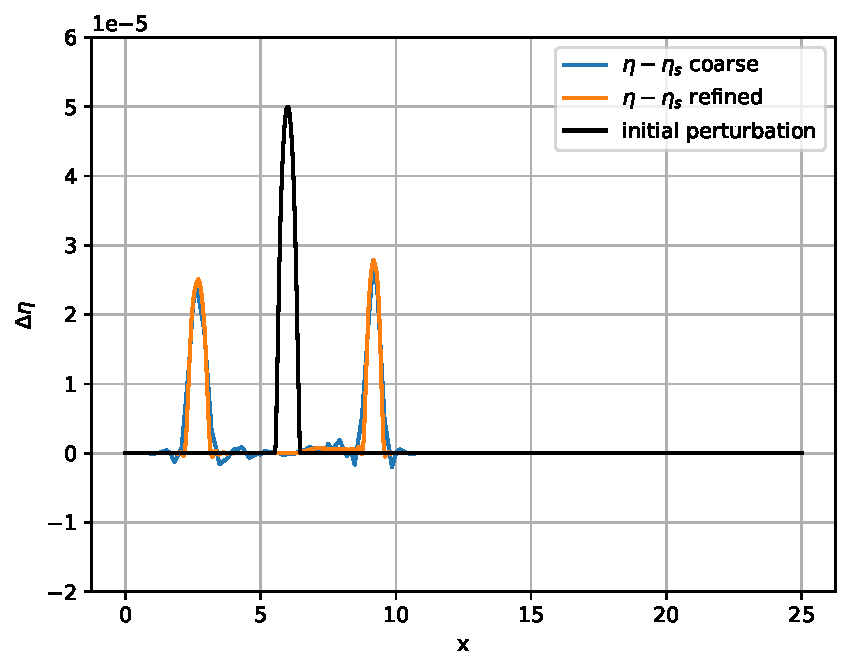
\includegraphics[width=\textwidth]{alb_latr_WBp3s14je.pdf}
         \caption{Jump e}
     \end{subfigure}
     \begin{subfigure}[b]{0.3\textwidth}
         \centering
         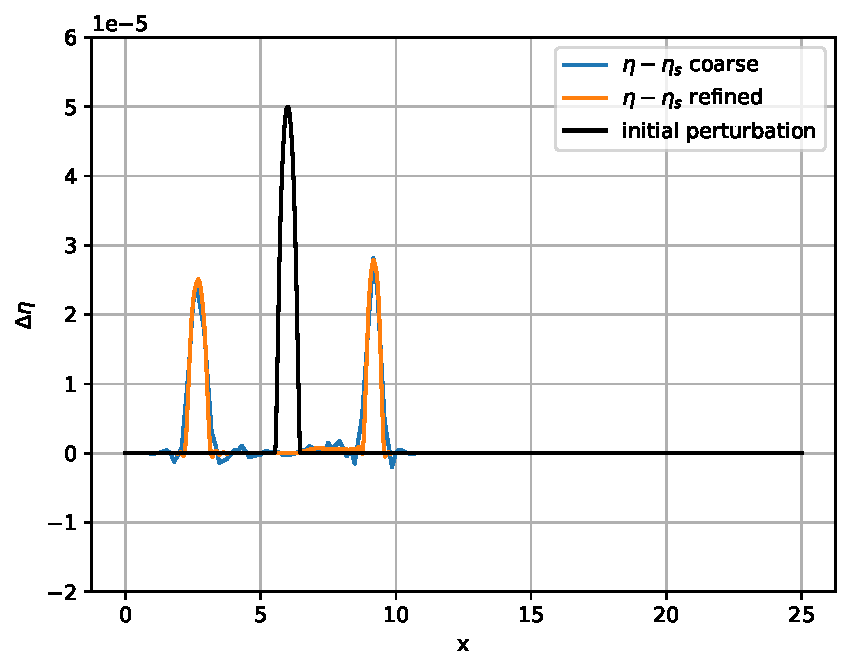
\includegraphics[width=\textwidth]{alb_latr_WBp3s14jr.pdf}
         \caption{Jump r}
     \end{subfigure}
        \label{pert_LatR_jumps}
\end{figure}


\end{frame}

\begin{frame}
\frametitle{Question}
\centering


What about the other steady states?


\end{frame}




\begin{frame}[label=NumericalResultsWithoutWBmonodimensionalcasesSW]
\frametitle{Convergence, PGL4}

\begin{figure}
     \centering
     \begin{subfigure}[b]{0.30\textwidth}
         \centering
         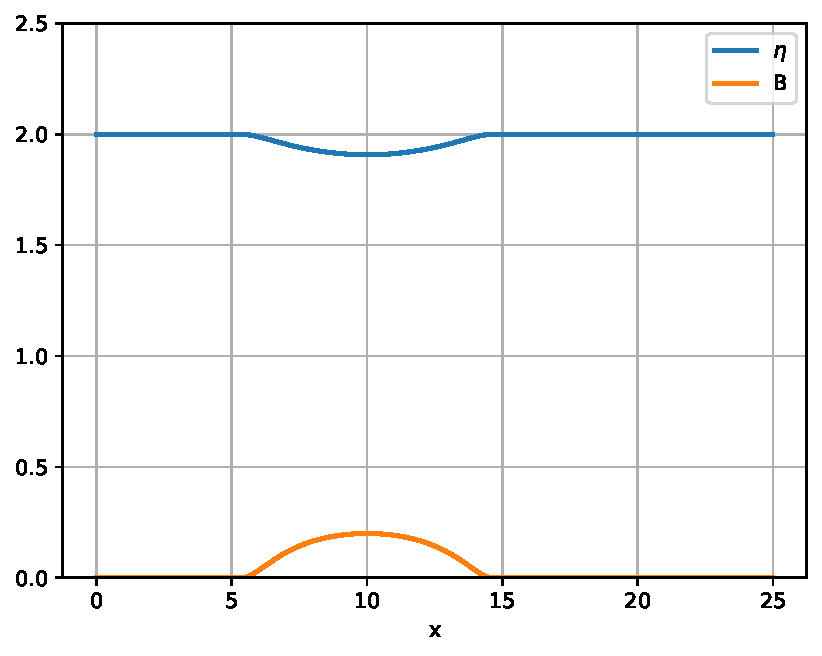
\includegraphics[width=\textwidth]{sub.pdf}
         %\caption{Subcritical, $(Hv)_L=4.42, \quad H_R=2$}
         \caption{Sub, $Hv\equiv 4.42$}
         \label{convergence_comp_jumps_sub}
     \end{subfigure}
     \begin{subfigure}[b]{0.30\textwidth}
         \centering
         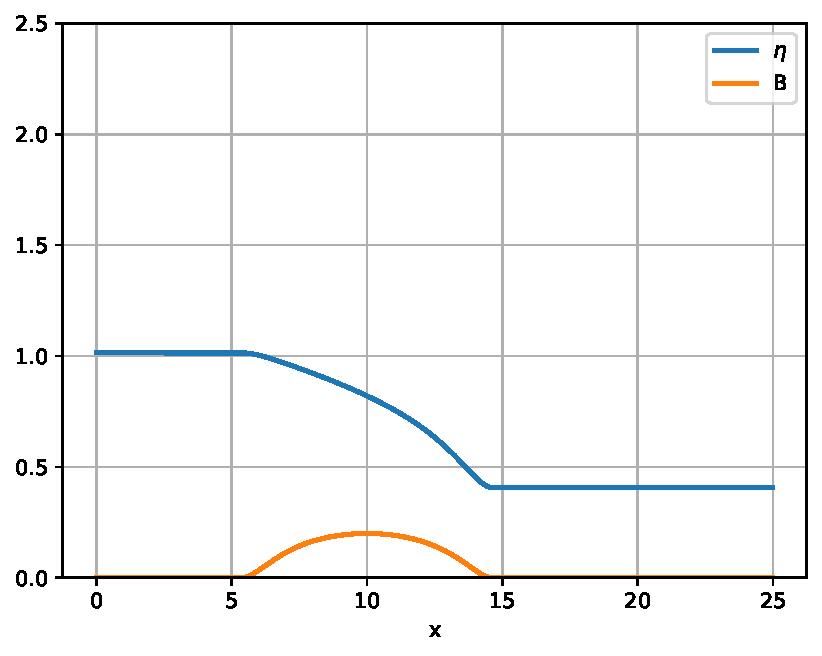
\includegraphics[width=\textwidth]{trans.pdf}
         %\caption{Transcritical, $(Hv)_L=1.53$}
         \caption{Trans, $Hv\equiv 1.53$}
         \label{convergence_comp_jumps_trans}
     \end{subfigure}
     \begin{subfigure}[b]{0.30\textwidth}
         \centering
         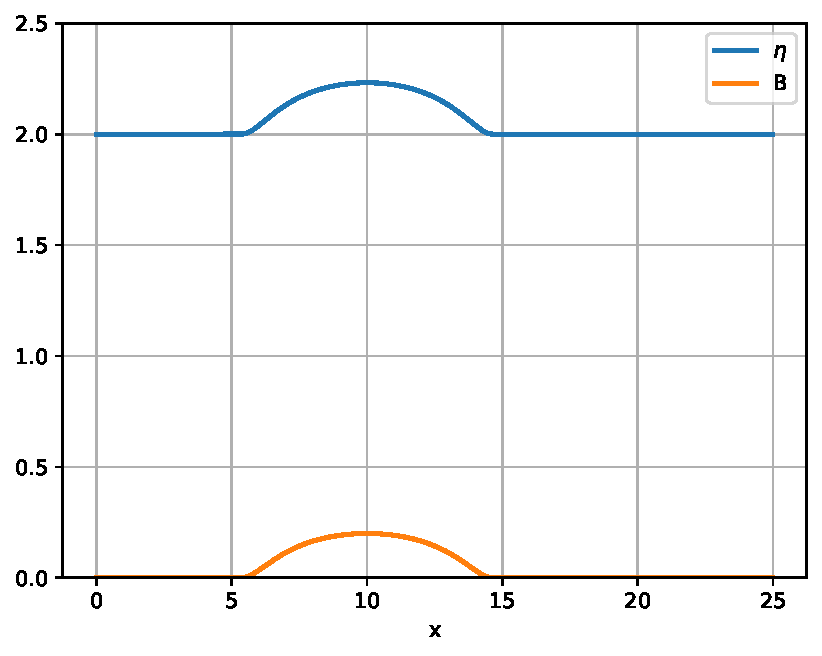
\includegraphics[width=\textwidth]{sup.pdf}
         %\caption{Supercritical, $(Hv)_L=24, \quad H_L=2$}
         \caption{Super, $Hv\equiv 24$}
         \label{convergence_comp_jumps_super}
     \end{subfigure}

        \label{convergence}
\end{figure}
\begin{figure}
     \centering
     \begin{subfigure}[b]{0.30\textwidth}
         \centering
         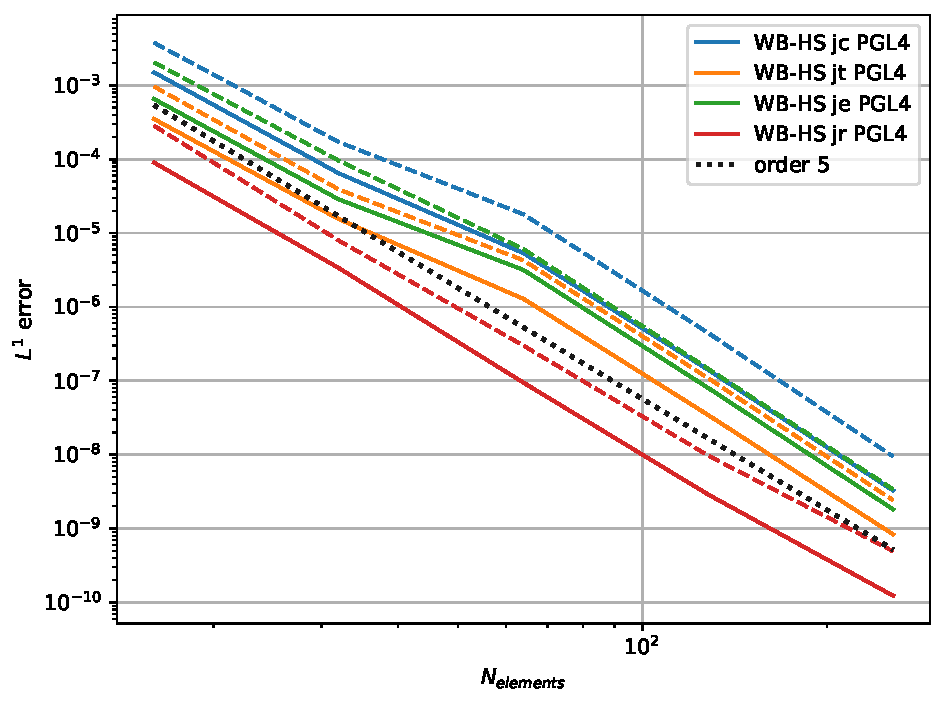
\includegraphics[width=\textwidth]{alb_sub_convergenceWB-HS.pdf}
         %\caption{Subcritical}
         \label{convergence_comp_jumps_sub}
     \end{subfigure}
     \begin{subfigure}[b]{0.30\textwidth}
         \centering
         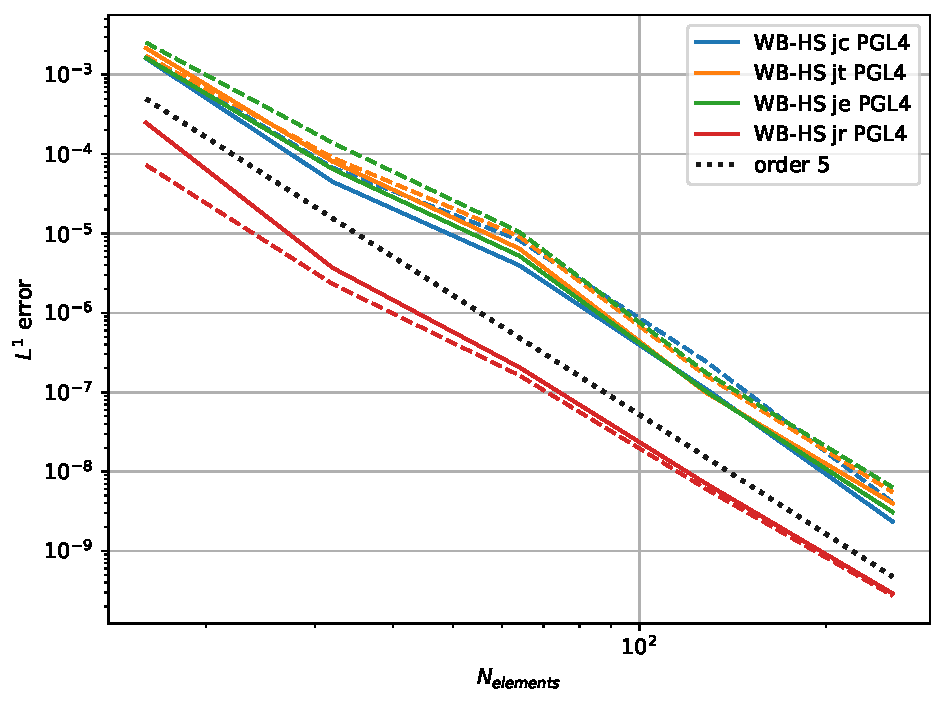
\includegraphics[width=\textwidth]{alb_trans_convergenceWB-HS.pdf}
         %\caption{Transcritical}
         \label{convergence_comp_jumps_trans}
     \end{subfigure}
     \begin{subfigure}[b]{0.30\textwidth}
         \centering
         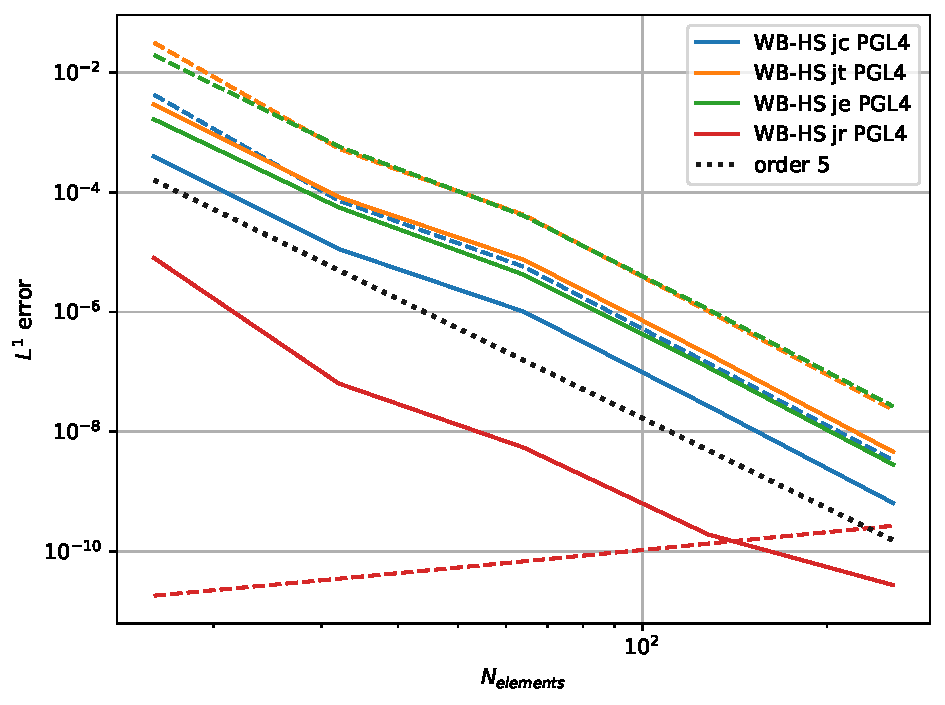
\includegraphics[width=\textwidth]{alb_sup_convergenceWB-HS.pdf}
         \label{convergence_comp_jumps_super}
     \end{subfigure}
        \caption*{Continuous $H$, Dashed $Hv$}

        \label{convergence}
\end{figure}

\end{frame}



\begin{frame}
\frametitle{Small perturbation}
\centering

\begin{figure}
     \centering
     \begin{subfigure}[b]{0.30\textwidth}
         \centering
         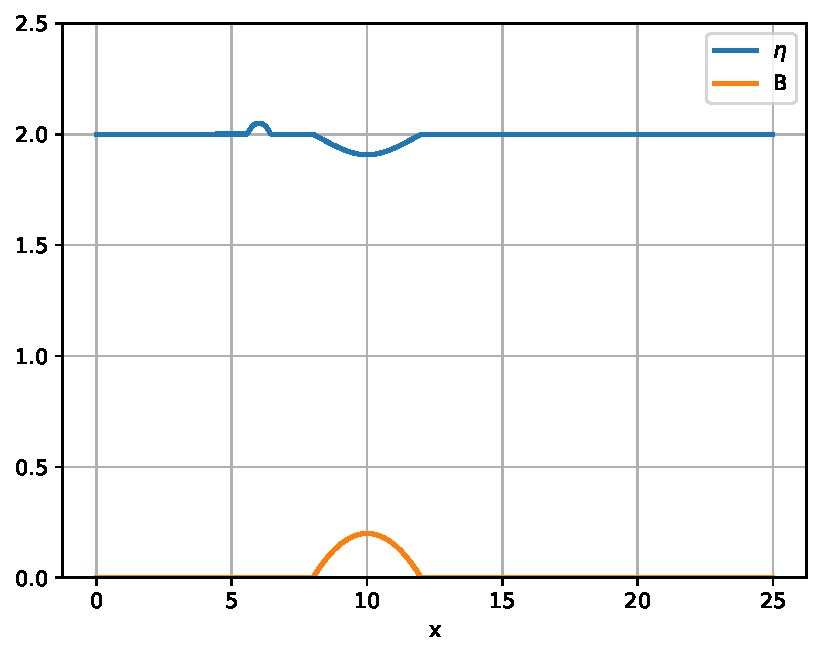
\includegraphics[width=\textwidth]{sub_not_smooth.pdf}
         \caption{Subcritical}
     \end{subfigure}
     \begin{subfigure}[b]{0.30\textwidth}
         \centering
         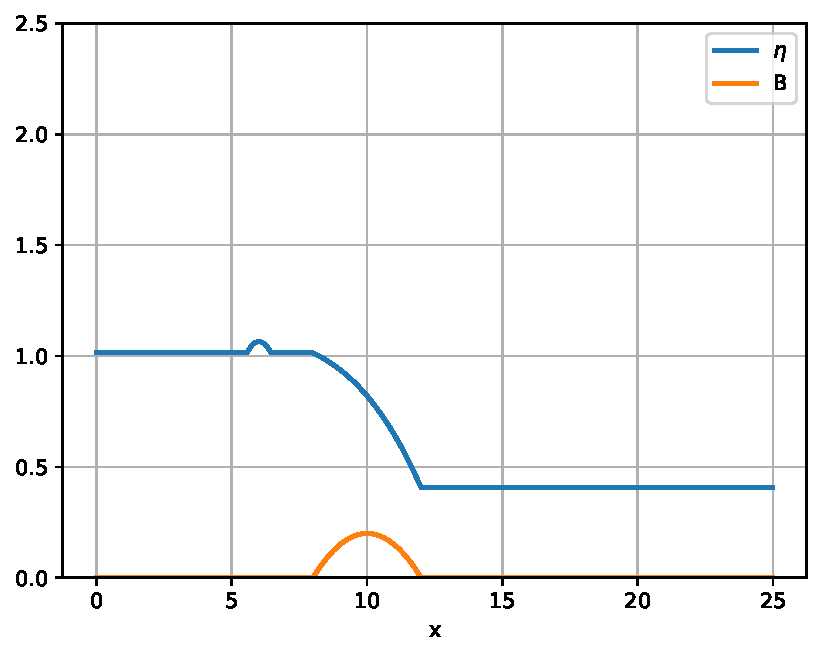
\includegraphics[width=\textwidth]{trans_not_smooth.pdf}
         \caption{Transcritical}
     \end{subfigure}
     \begin{subfigure}[b]{0.30\textwidth}
         \centering
         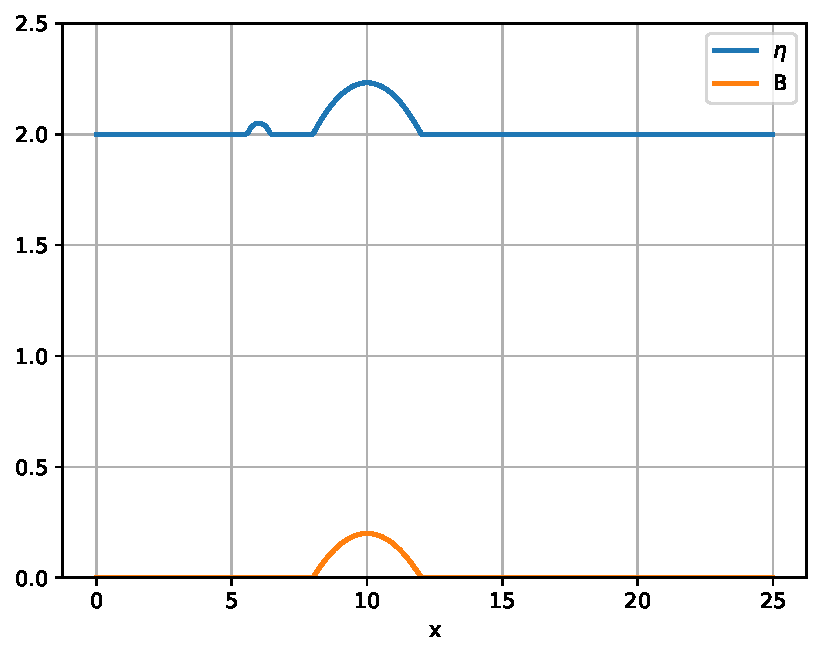
\includegraphics[width=\textwidth]{sup_not_smooth.pdf}
         \caption{Supercritical}
     \end{subfigure}
         \caption{Perturbation amplified by $1000$}

        \label{convergence}
\end{figure}



\end{frame}



\begin{frame}
\frametitle{Supercritical}
\begin{figure}
     \centering
     \begin{subfigure}[b]{0.28\textwidth}
         \centering
         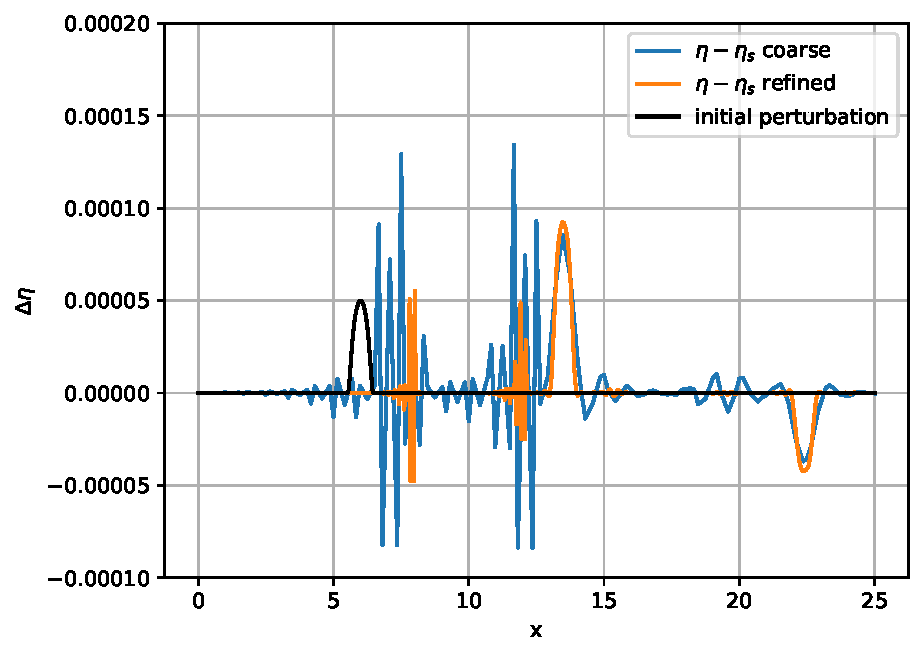
\includegraphics[width=\textwidth]{alb_sup_WBp3s14jc.pdf}
         \caption{Jump c}
     \end{subfigure}
     %\hfill
     \begin{subfigure}[b]{0.28\textwidth}
         \centering
         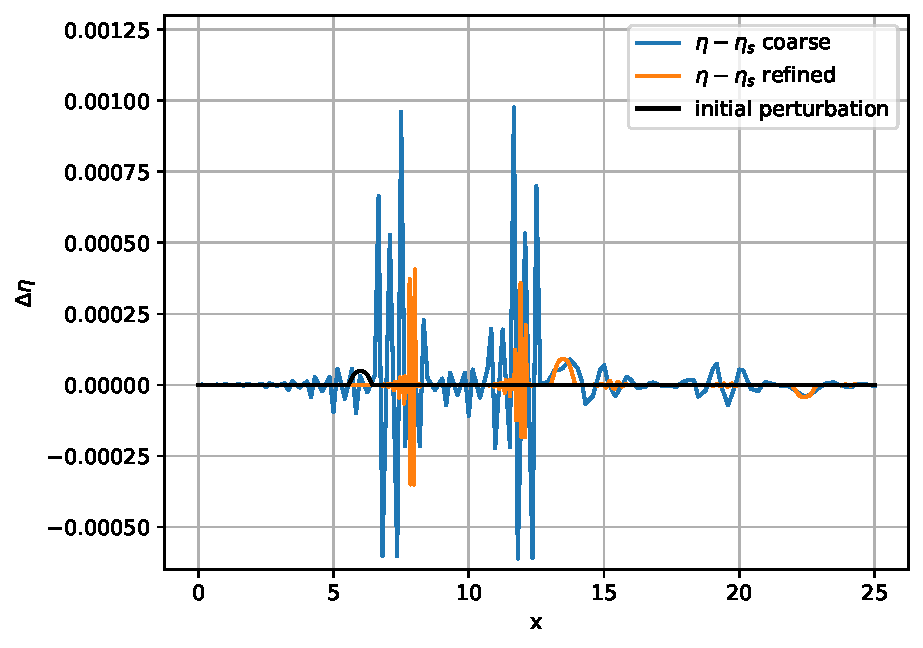
\includegraphics[width=\textwidth]{alb_sup_WBp3s14jt.pdf}
         \caption{Jump t}
     \end{subfigure}
     \vskip\baselineskip
     \begin{subfigure}[b]{0.28\textwidth}
         \centering
         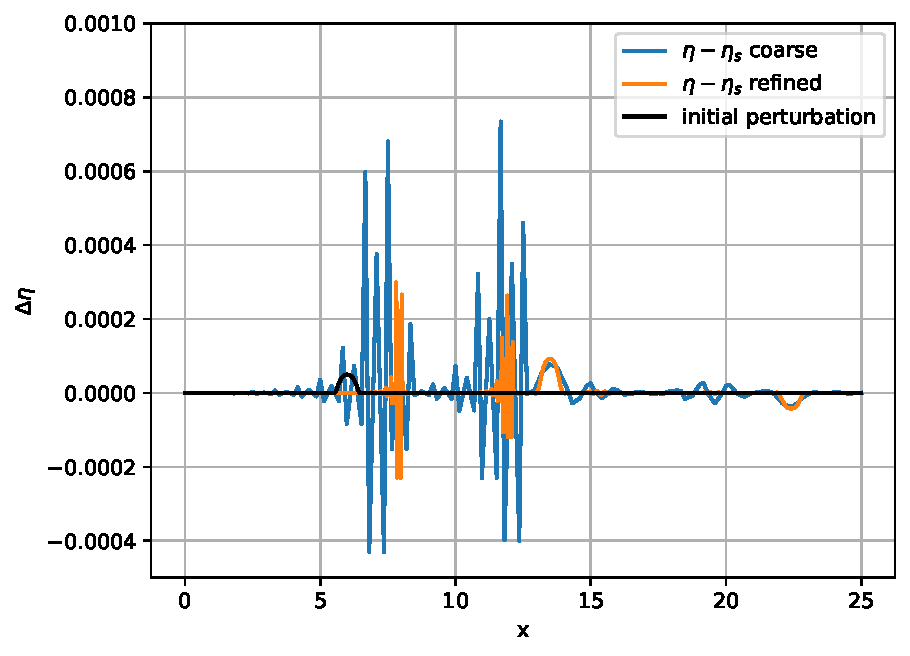
\includegraphics[width=\textwidth]{alb_sup_WBp3s14je.pdf}
         \caption{Jump e}
     \end{subfigure}
     \begin{subfigure}[b]{0.28\textwidth}
         \centering
         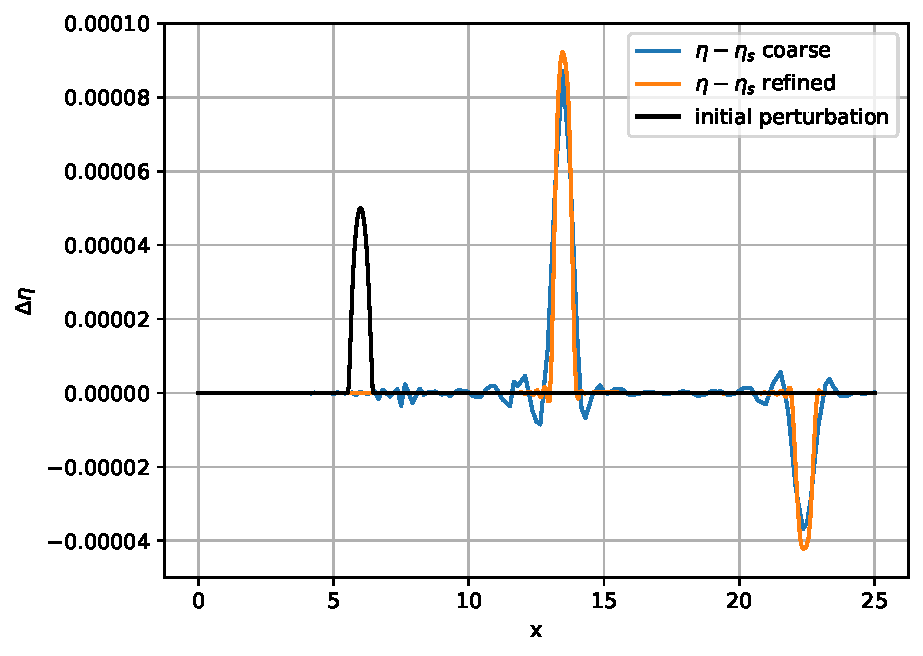
\includegraphics[width=\textwidth]{alb_sup_WBp3s14jr.pdf}
         \caption{Jump r}
     \end{subfigure}
        \label{pert_super_jumps}
\end{figure}
\end{frame}


\begin{frame}
\frametitle{Supercritical}
\begin{figure}
     \centering
     \begin{subfigure}[b]{0.28\textwidth}
         \centering
         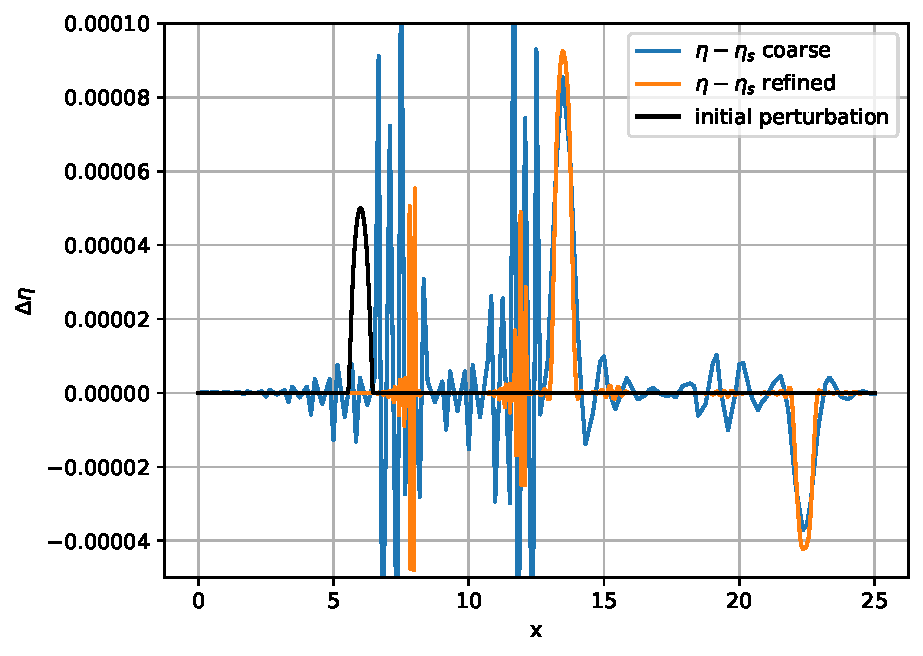
\includegraphics[width=\textwidth]{alb_sup_same_scale_WBp3s14jc.pdf}
         \caption{Jump c}
     \end{subfigure}
     %\hfill
     \begin{subfigure}[b]{0.28\textwidth}
         \centering
         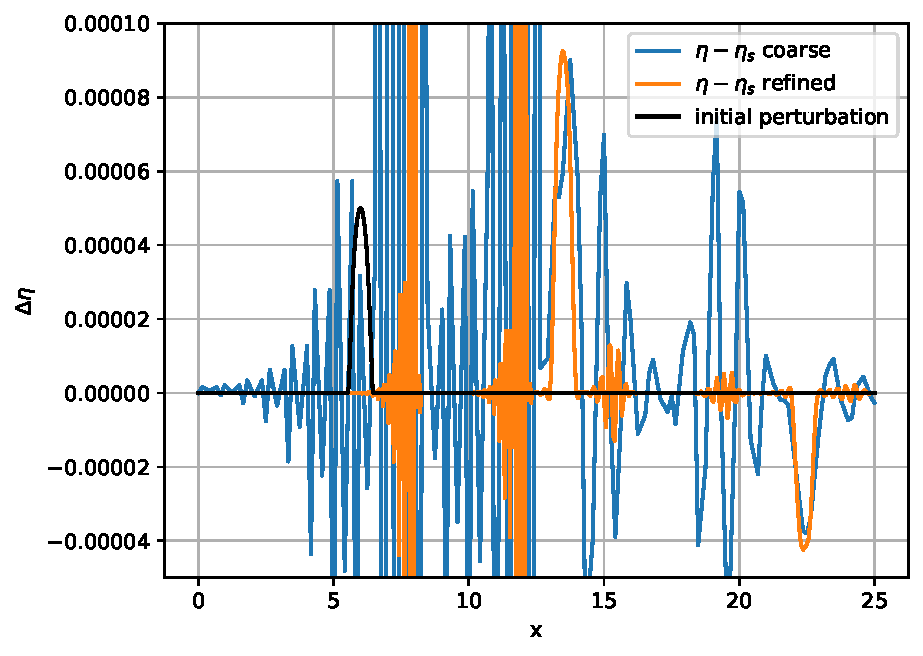
\includegraphics[width=\textwidth]{alb_sup_same_scale_WBp3s14jt.pdf}
         \caption{Jump t}
     \end{subfigure}
     \vskip\baselineskip
     \begin{subfigure}[b]{0.28\textwidth}
         \centering
         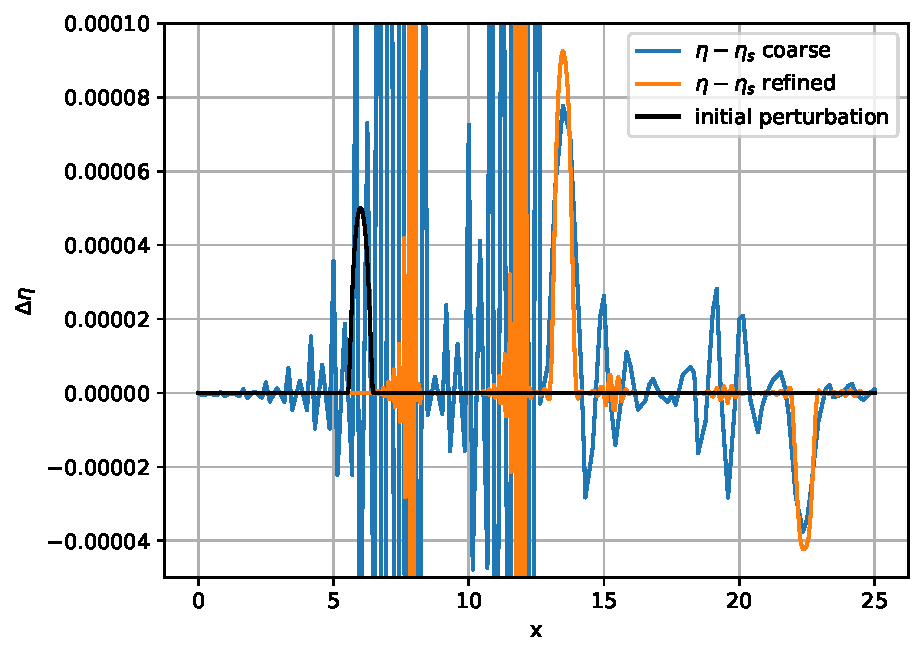
\includegraphics[width=\textwidth]{alb_sup_same_scale_WBp3s14je.pdf}
         \caption{Jump e}
     \end{subfigure}
     \begin{subfigure}[b]{0.28\textwidth}
         \centering
         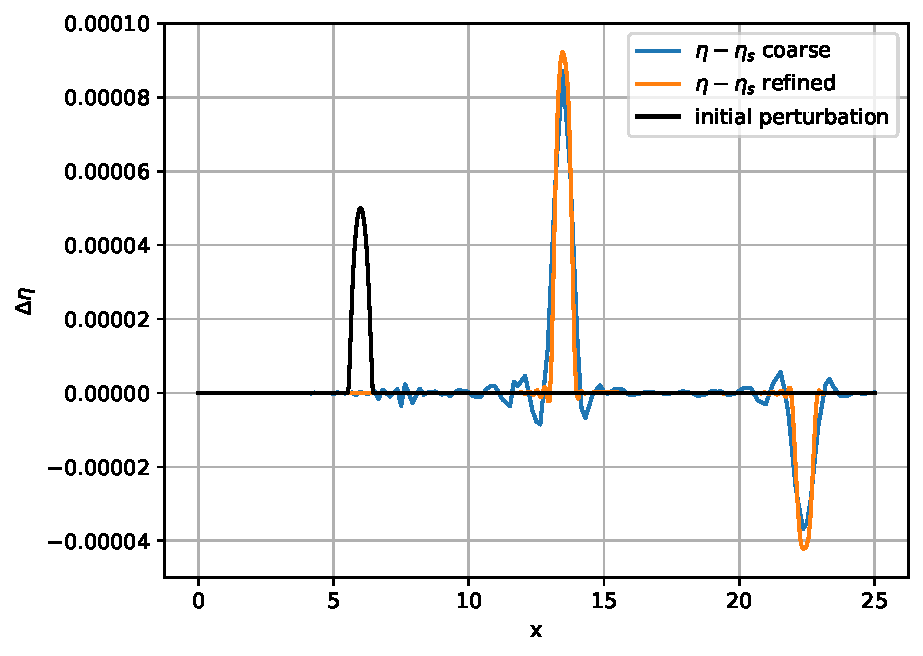
\includegraphics[width=\textwidth]{alb_sup_same_scale_WBp3s14jr.pdf}
         \caption{Jump r}
     \end{subfigure}
        \label{pert_super_jumps}
\end{figure}
\end{frame}



\begin{frame}
\frametitle{Analogous results}


Analogous results for...

\end{frame}

\begin{frame}
\frametitle{Analogous results}

\begin{itemize}

\item for other basis functions (Bn, Pn and PGLn)
\begin{figure}
     \centering
     \begin{subfigure}[b]{0.3\textwidth}
         \centering
         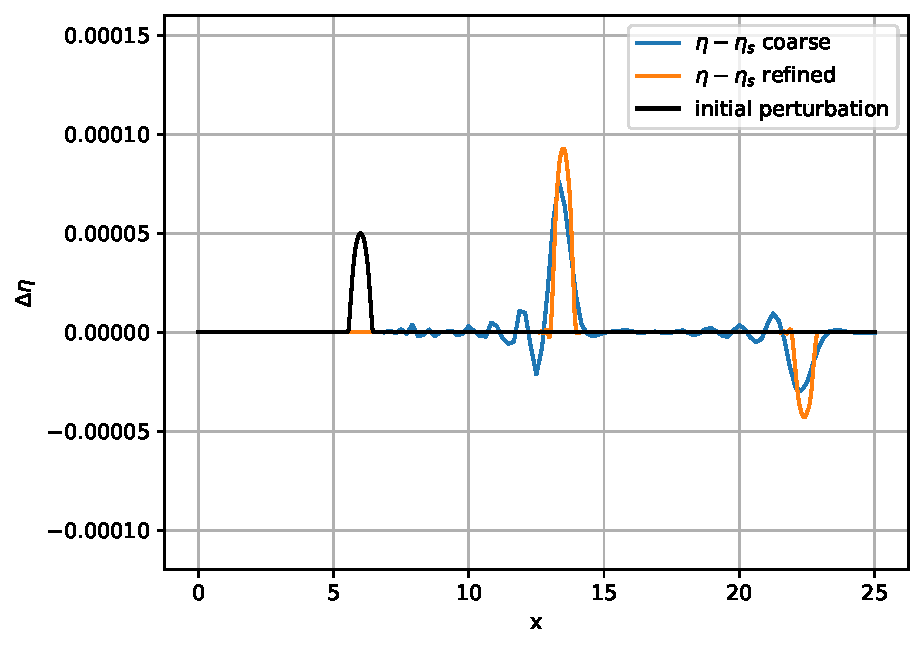
\includegraphics[width=\textwidth]{alb_bases_WBp3s14jrPGL2.pdf}
         \caption{PGL2}
     \end{subfigure}
     \begin{subfigure}[b]{0.3\textwidth}
         \centering
         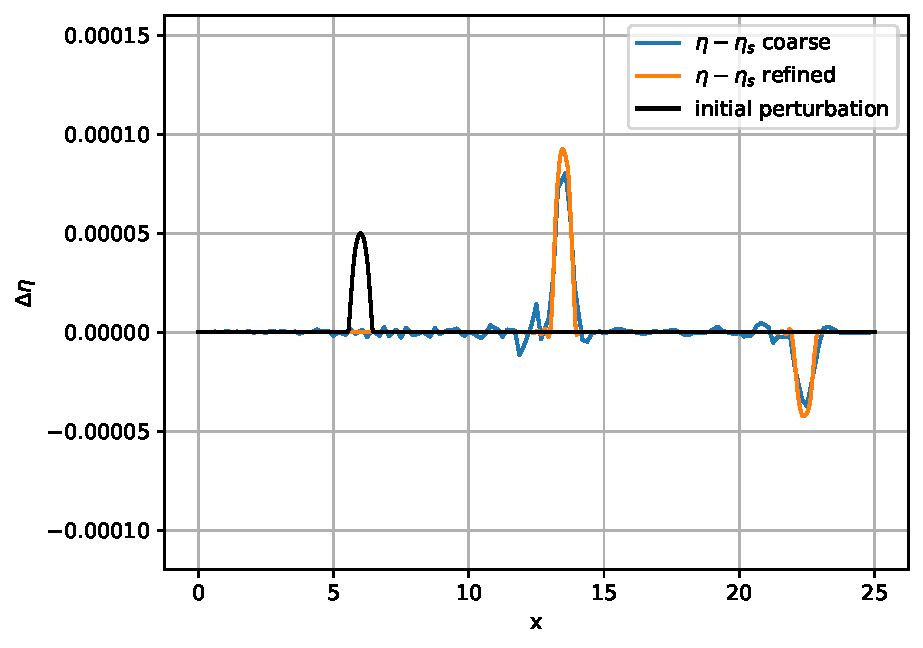
\includegraphics[width=\textwidth]{alb_bases_WBp3s14jrPGL3.pdf}
         \caption{PGL3}
     \end{subfigure}
     \begin{subfigure}[b]{0.3\textwidth}
         \centering
         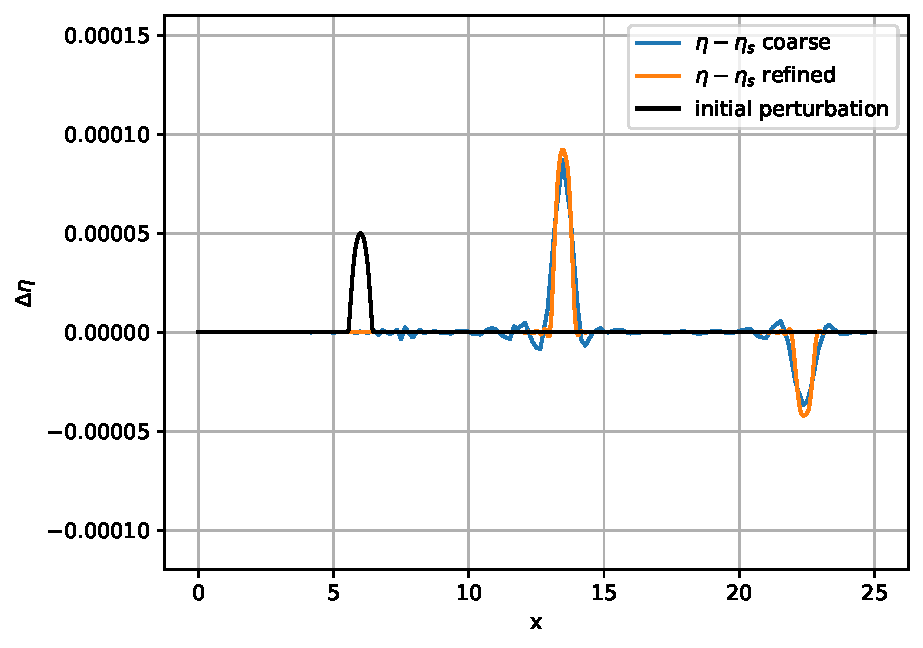
\includegraphics[width=\textwidth]{alb_bases_WBp3s14jrPGL4.pdf}
         \caption{PGL4}
     \end{subfigure}
        \caption*{Supercritical: "fair" comparison with $60$, $40$ and $30$ elements}
        \label{convergence}
\end{figure}

\centering
(Constant number of DoFs)

\end{itemize}

\end{frame}



\begin{frame}
\frametitle{Analogous results}

\begin{itemize}
\item for other tests 
\begin{figure}
     \centering
     \begin{subfigure}[b]{0.4\textwidth}
         \centering
         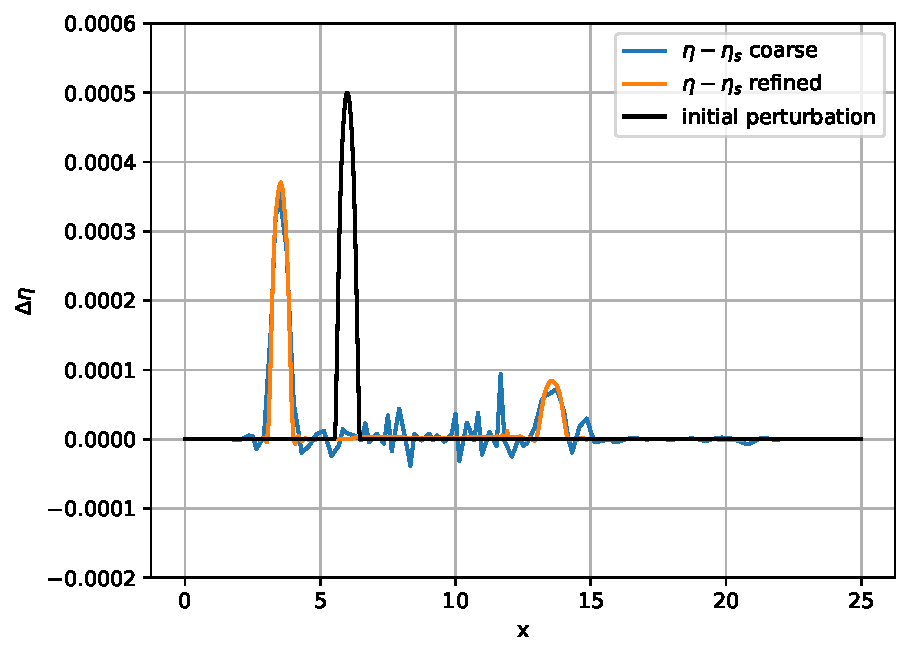
\includegraphics[width=\textwidth]{alb_trans_WBp2s14jr.pdf}
         \caption{Transcritical}
     \end{subfigure}
     %\hfill
     \begin{subfigure}[b]{0.4\textwidth}
         \centering
         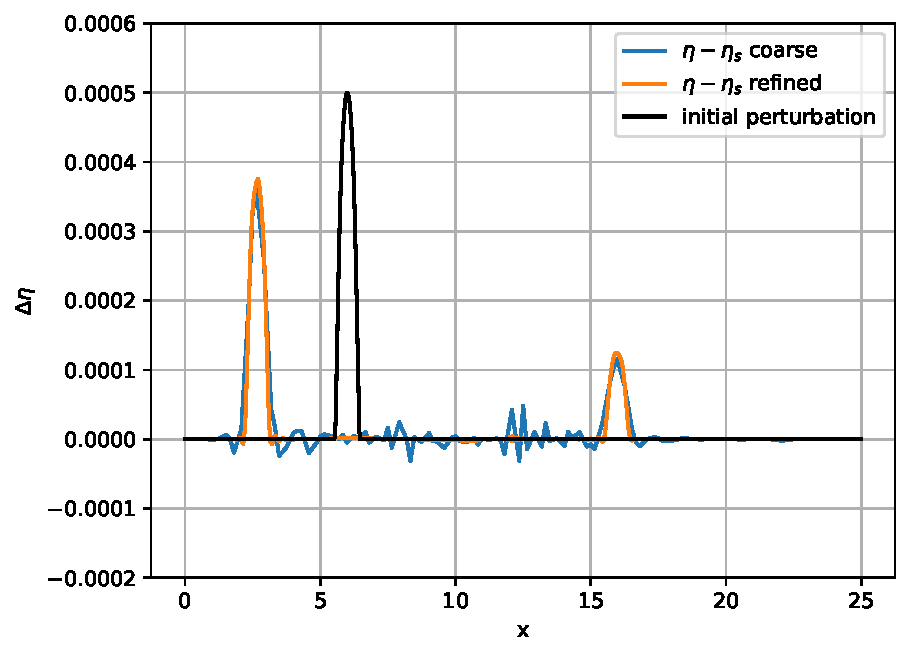
\includegraphics[width=\textwidth]{alb_sub_WBp2s14jr.pdf}
         \caption{Subcritical}
     \end{subfigure}
\end{figure}

\end{itemize}





\centering
(NB: No limiting at all)

\end{frame}

\begin{frame}
\frametitle{Analogous results}

\begin{itemize}

\item with friction
$$
\boldsymbol{S}(x,\uvec{u})=-\begin{pmatrix}
0\\
gH\frac{\partial}{\partial x} \textcolor{black}{B}
\end{pmatrix}-\textcolor{red}{g\frac{n^2\vert Hv \vert}{H^{\frac{7}{3}}} \begin{pmatrix}
0\\
Hv
\end{pmatrix}}
$$



\begin{figure}
     \centering
     \begin{subfigure}[b]{0.4\textwidth}
         \centering
         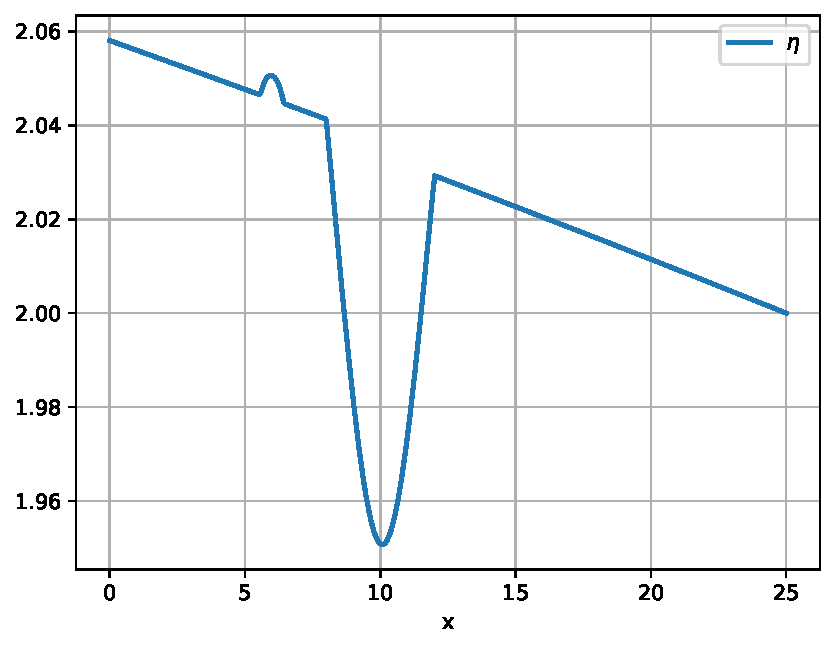
\includegraphics[width=\textwidth]{friction/friction_sub.pdf}
     \end{subfigure}
     \begin{subfigure}[b]{0.4\textwidth}
         \centering
         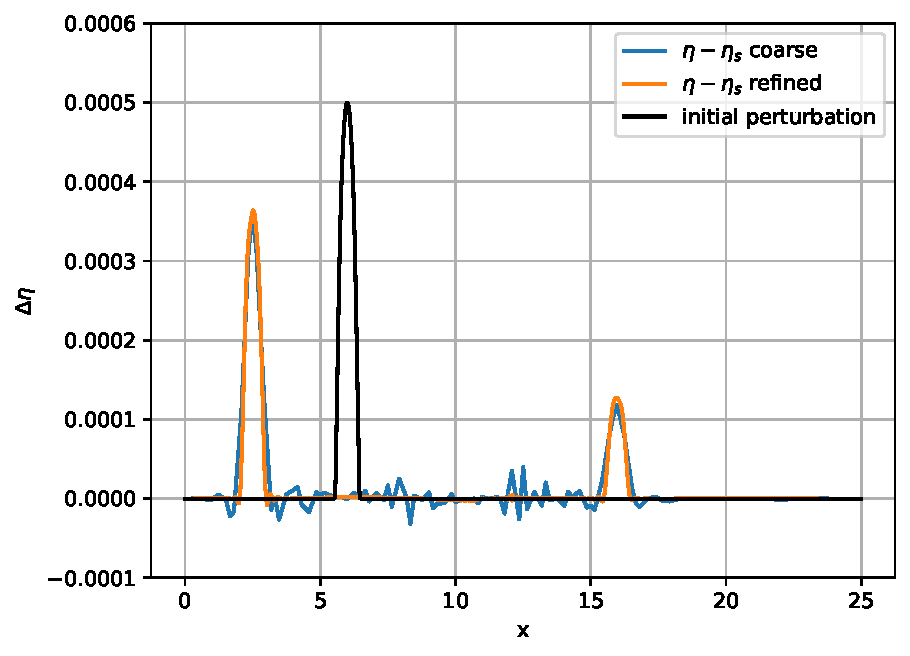
\includegraphics[width=\textwidth]{alb_sub_fri_WBp2s14jr.pdf}
     \end{subfigure}
         \caption*{Subcritical: perturbation amplified by $100$}
        \label{pert_trans_sup}
\end{figure}
\centering
(Same for supercritical)









\end{itemize}

\end{frame}


%\begin{frame}
%\frametitle{Further}
%
%Other WB space discretizations and stabilizations: Global flux
%
%
%\centering
%
%
%\begin{align*}
%\centering
%\frac{\partial}{\partial t}\uvec{u} +\frac{\partial}{\partial x}&  \boldsymbol{F} =\boldsymbol{S}\\
% & \Downarrow ~{\footnotesize \uvec{R}=-\int^x_{x_L} \boldsymbol{S},\quad \boldsymbol{G}=\boldsymbol{F}+\uvec{R} } & \\
% \frac{\partial}{\partial t}\uvec{u} +\frac{\partial}{\partial x}&  \textcolor{red}{\boldsymbol{G}} =\uvec{0}  
%\end{align*}
%
%
%$$\textcolor{blue}{\textbf{ST}_i(\uapp)}=\sum_{f}\alpha_f  \biggl\llbracket \boldsymbol{J} \frac{\partial}{\partial x} \varphi_i\biggr\rrbracket \vert \boldsymbol{J} \vert^{-1}  \biggl\llbracket \frac{\partial}{\partial x} \textcolor{red}{\uvec{G}} \biggr\rrbracket$$
%
%\end{frame}




\begin{frame}[label=NumericalResultsWithoutWBmonodimensionalcasesSW]
\frametitle{Global flux, $\boldsymbol{G}=\boldsymbol{F}-\int^x_{x_L} \boldsymbol{S}$}

\begin{figure}
     \centering
     \begin{subfigure}[b]{0.30\textwidth}
         \centering
         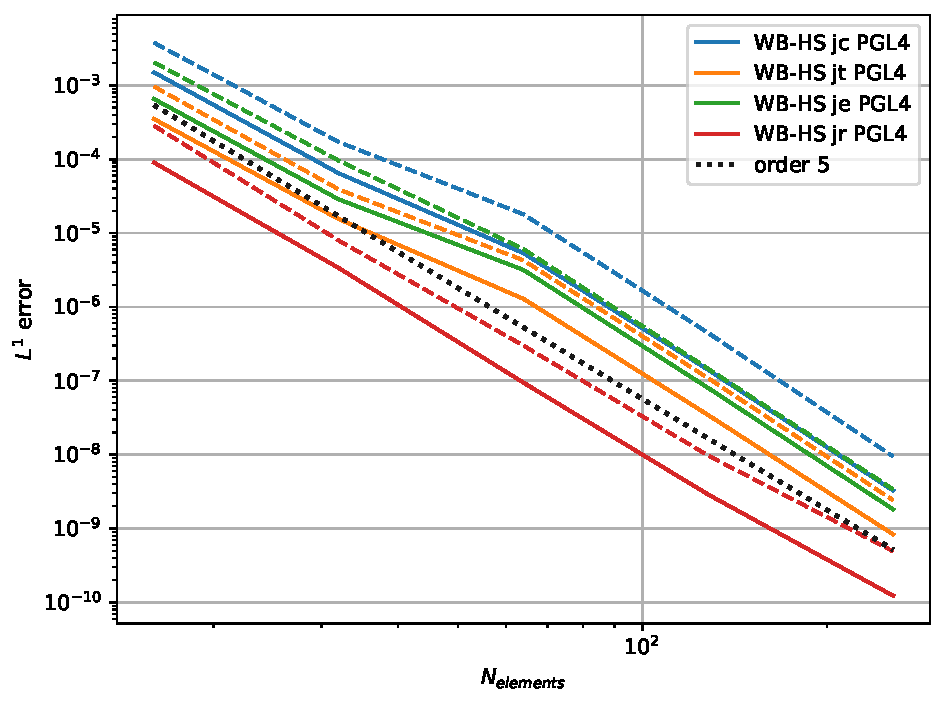
\includegraphics[width=\textwidth]{alb_sub_convergenceWB-HS.pdf}
         \caption{Subcritical}
         \label{convergence_comp_jumps_sub}
     \end{subfigure}
     \begin{subfigure}[b]{0.30\textwidth}
         \centering
         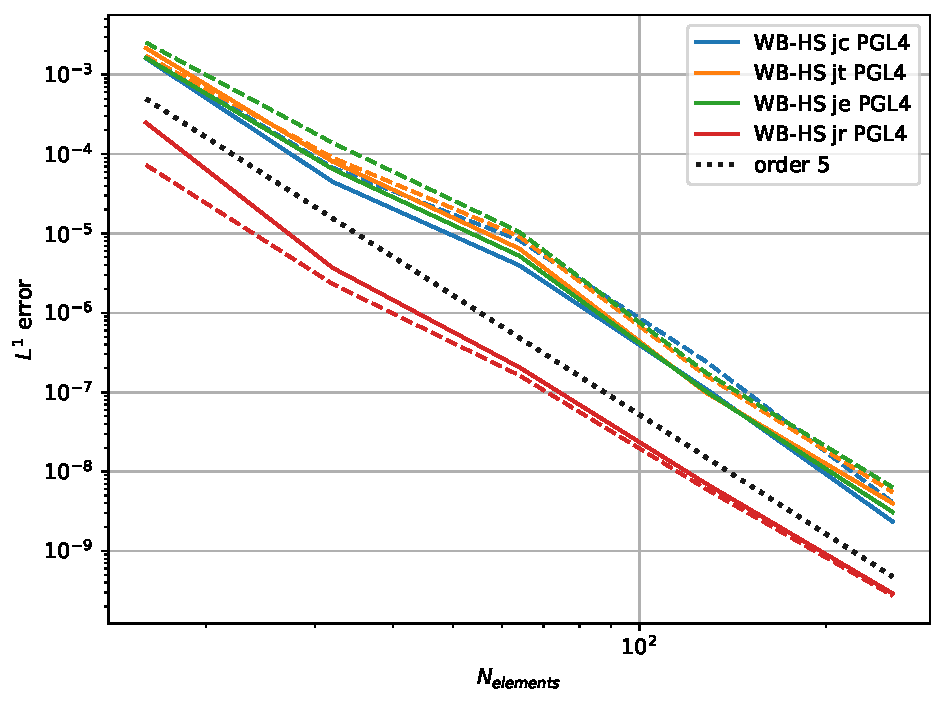
\includegraphics[width=\textwidth]{alb_trans_convergenceWB-HS.pdf}
         \caption{Transcritical}
         \label{convergence_comp_jumps_trans}
     \end{subfigure}
     \begin{subfigure}[b]{0.30\textwidth}
         \centering
         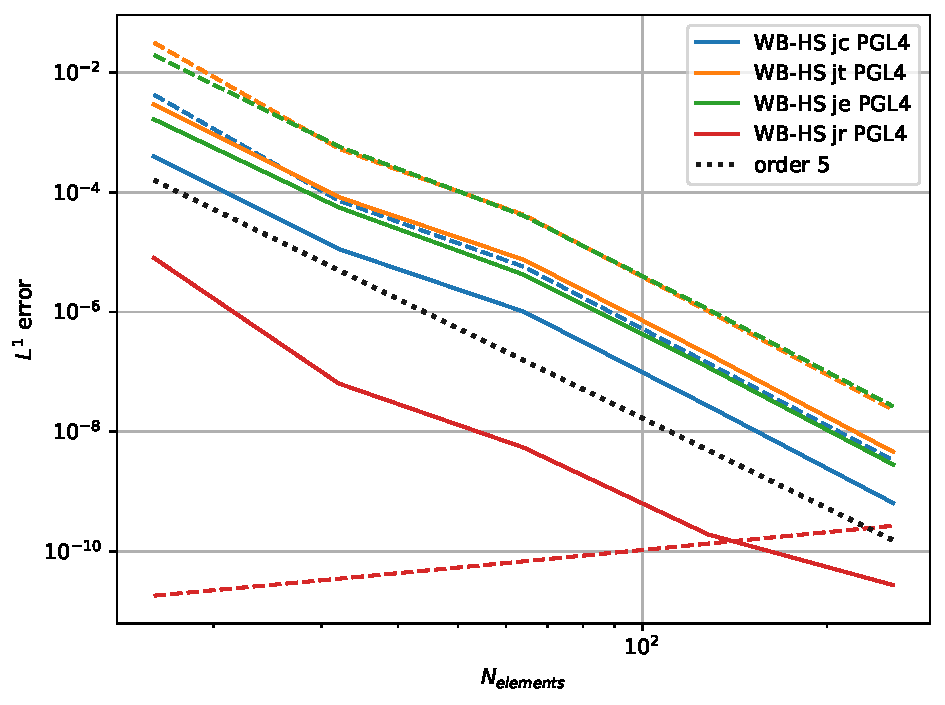
\includegraphics[width=\textwidth]{alb_sup_convergenceWB-HS.pdf}
		\caption{Supercritical}              
         \label{convergence_comp_jumps_super}
     \end{subfigure}
\end{figure}
%
\begin{figure}
     \centering
     \begin{subfigure}[b]{0.30\textwidth}
         \centering
         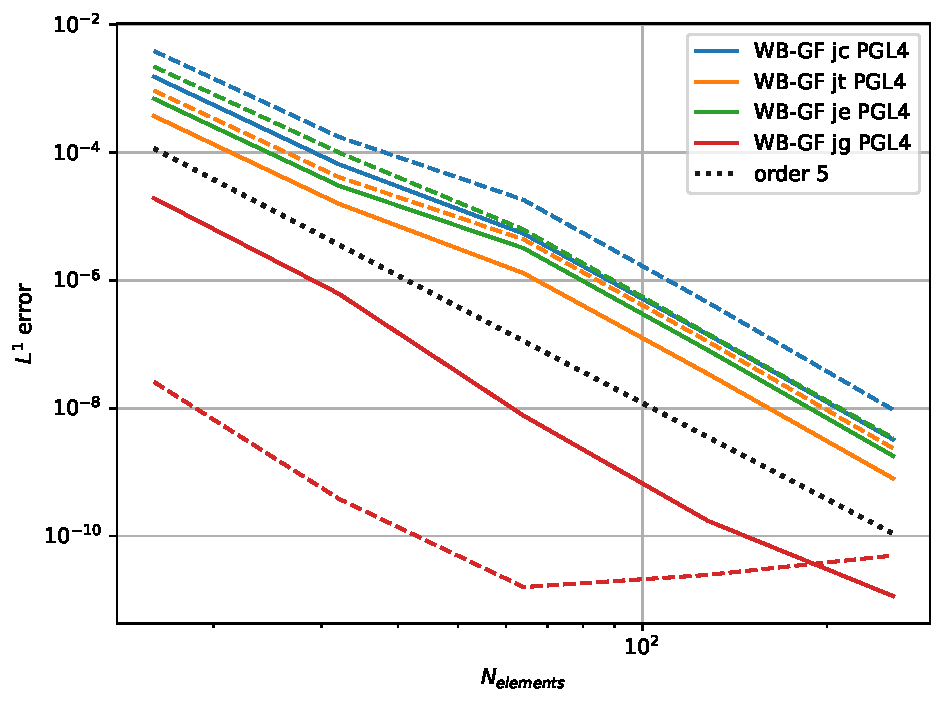
\includegraphics[width=\textwidth]{alb_sub_convergenceWB-GF.pdf}
         %\caption{Subcritical}
         \label{convergence_comp_jumps_sub}
     \end{subfigure}
     \begin{subfigure}[b]{0.30\textwidth}
         \centering
         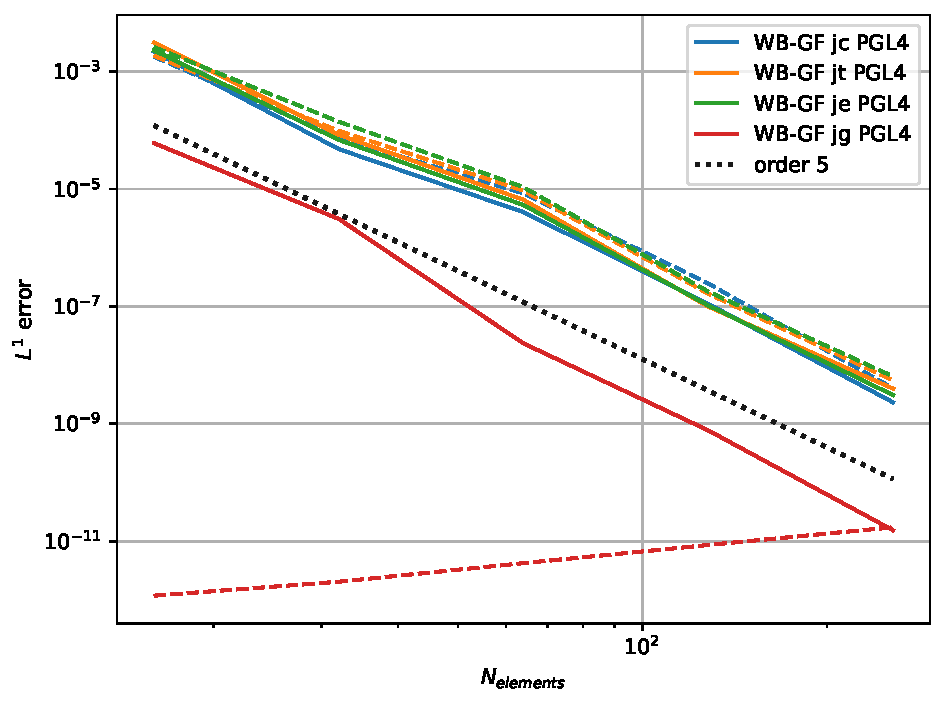
\includegraphics[width=\textwidth]{alb_trans_convergenceWB-GF.pdf}
         %\caption{Transcritical}
         \label{convergence_comp_jumps_trans}
     \end{subfigure}
     \begin{subfigure}[b]{0.30\textwidth}
         \centering
         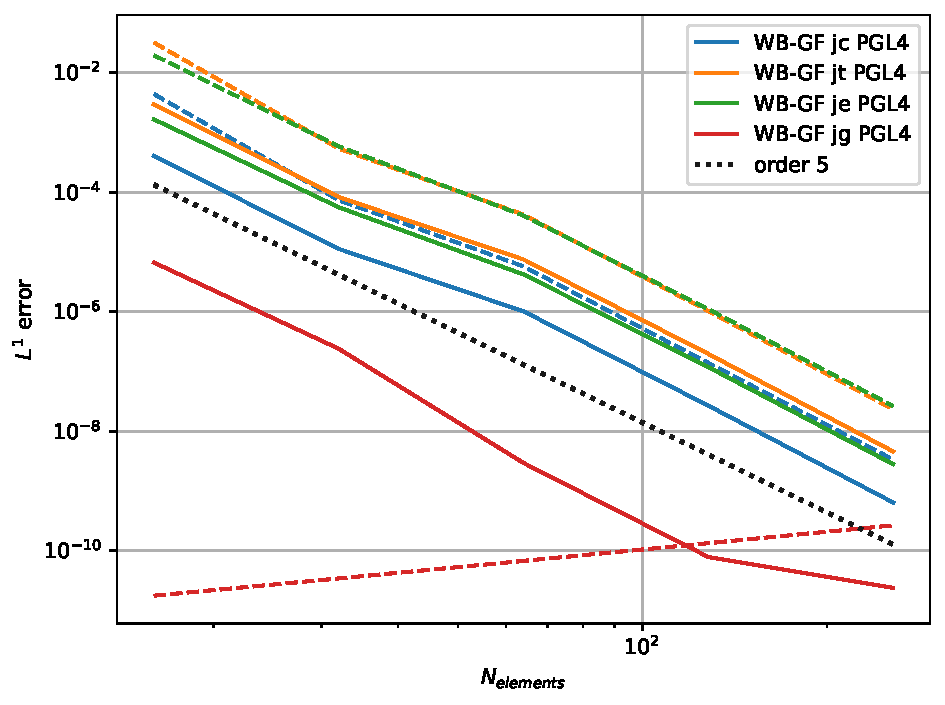
\includegraphics[width=\textwidth]{alb_sup_convergenceWB-GF.pdf}
         %\caption{Supercritical}
         \label{convergence_comp_jumps_super}
     \end{subfigure}
\end{figure}

\end{frame}



\section*{Conclusions}
\frame\sectionpage


\begin{frame}[label=Conclusions]
\frametitle{Conclusions}
\begin{itemize}
\visible<2->{\item WB space discretization (w.r.t. lake at rest)}
\visible<3->{\item Three new well-balanced CIP stabilizations
\begin{itemize}
\item jt (total height)
\item je (entropy variables)
\item \textcolor{red}{jr (residual)}
\end{itemize}

}
\visible<4->{\item The numerical results confirm 
\begin{itemize}
\item Exact well-balancing for lake at rest
\item HO accuracy 
\item \textcolor{red}{Ability of jr to handle general steady states}
\end{itemize}}

\end{itemize}
\end{frame}


\begin{frame}[label=THEEND]
\frametitle{The End}
  \centering {\Huge
  \textbf{\emph{Thank you\footnote{Looking for a postdoc position in the U.S.}}}}

\vspace{2em}

{\footnotesize
Novel well-balanced continuous interior penalty stabilizations;\\ Micalizzi, Ricchiuto, Abgrall; 2023}

\end{frame}




\begin{frame}[label=SW]
\frametitle{Shallow water equations, Eulerian}
%We will mainly focus on

$$\frac{\partial}{\partial t}\uvec{u}+\frac{\partial}{\partial x} \boldsymbol{F}(\uvec{u})=\boldsymbol{S}(x,\uvec{u}), \quad (x,t)\in \Omega \times [0,T], ~\Omega:=(x_L,x_R)$$

    \begin{columns}

        \begin{column}{0.50\textwidth}
$$
\uvec{u}:=\begin{pmatrix}
H\\
Hv\\
\end{pmatrix}$$
$$\uvec{F}(\uvec{u}):=\begin{pmatrix}
Hv\\
Hv^2+\textcolor{SSCdarkgreen}{g}\frac{H^2}{2}
\end{pmatrix}$$
$$
\boldsymbol{S}(x,\uvec{u}):=-\begin{pmatrix}
0\\
gH\frac{\partial}{\partial x} \textcolor{magenta}{B}(x)
\end{pmatrix}
$$

        \end{column}
        \begin{column}{0.50\textwidth}

	\begin{figure}
		\centering
		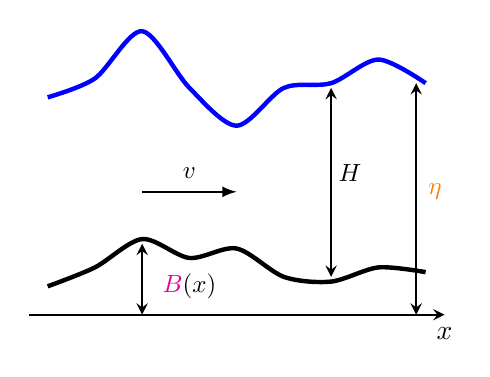
\begin{tikzpicture}[thick, scale=1.2]
			
			\draw [-stealth] (-0.2,-0.3) -- (4.2,-0.3);
			\node [black,scale=1] at (4.2,-0.5) {$x$};
			
			\draw [stealth-stealth] (1,-0.3) -- (1,0.45);
			\node [black,scale=0.9] at (1.5,0) {$\textcolor{magenta}{B}(x)$};
			\draw [stealth-stealth] (3,0.1) -- (3,2.1);
			\node [black,scale=0.9] at (3.2,1.2) {$H$};
			\draw [stealth-stealth] (3.9,-0.3) -- (3.9,2.15);
			\node [black,scale=0.9] at (4.1,1.0) {$\textcolor{orange}{\eta}$};
			
			\draw [-latex] (1,1) -- (2,1);
			\node [black,scale=0.9] at (1.5,1.2) {$v$};
			
			\draw [black,ultra thick] plot [smooth] coordinates {(0,0) (0.5,0.2) (1,0.5) (1.5,0.3) (2,0.4) (2.5,0.1) (3,0.05) (3.5,0.2) (4,0.15)};
			\draw [blue, ultra thick]  plot [smooth] coordinates {(0,2) (0.5,2.2) (1,2.7) (1.5,2.1) (2,1.7) (2.5,2.1) (3,2.15) (3.5,2.4) (4,2.15)};
			
		\end{tikzpicture}
		
	\end{figure}

        \end{column}
    \end{columns}


\centering
\vspace{1em}
$$\textcolor{orange}{\eta}:=H+B$$      

\end{frame}


\begin{frame}
\frametitle{Shallow water equations, simplification of Euler (with gravity)}

$$\frac{\partial}{\partial t}\uvec{u}+\frac{\partial}{\partial x} \boldsymbol{F}(\uvec{u})=\boldsymbol{S}(x,\uvec{u}), \quad (x,t)\in \Omega \times [0,T], ~\Omega:=(x_L,x_R)$$

    \begin{columns}

        \begin{column}{0.50\textwidth}
$$
\uvec{u}:=\begin{pmatrix}
H\\
Hv\\
\end{pmatrix}$$
$$\uvec{F}(\uvec{u}):=\begin{pmatrix}
Hv\\
Hv^2+\textcolor{SSCdarkgreen}{g}\frac{H^2}{2}
\end{pmatrix}$$
$$
\boldsymbol{S}(x,\uvec{u}):=-\begin{pmatrix}
0\\
gH\frac{\partial}{\partial x} \textcolor{magenta}{B}(x)
\end{pmatrix}
$$

        \end{column}
        \begin{column}{0.50\textwidth}

\begin{align*}
H &\sim \rho\\
p &\sim \textcolor{SSCdarkgreen}{g}\frac{H^2}{2}\\
B(x) &\sim \phi(x)
\end{align*}


Neglecting the energy equation

        \end{column}
    \end{columns}



\end{frame}



\end{document}

